\documentclass[12pt,a4paper]{article}

% Packages
\usepackage[utf8]{inputenc}
\usepackage[italian]{babel}
\usepackage{graphicx}
\usepackage{booktabs}
\usepackage{amsmath}
\usepackage{amssymb}
\usepackage{hyperref}
\usepackage{listings}
\usepackage{xcolor}
\usepackage{algorithm2e}
\usepackage{subcaption}
\usepackage{float}
\usepackage{geometry}
\usepackage{fancyhdr}
\usepackage{titlesec}
\usepackage{enumitem}

% TikZ per diagrammi
\usepackage{tikz}
\usetikzlibrary{shapes,arrows,positioning,fit,backgrounds,calc}

% Page setup
\geometry{margin=2.5cm}
\pagestyle{fancy}
\fancyhf{}
\fancyhead[L]{\leftmark}
\fancyhead[R]{ResQPet}
\fancyfoot[C]{\thepage}

% Code listing style
\lstdefinestyle{python}{
    language=Python,
    basicstyle=\ttfamily\small,
    keywordstyle=\color{blue}\bfseries,
    stringstyle=\color{red},
    commentstyle=\color{green!60!black},
    morecomment=[l][\color{magenta}]{\#},
    numbers=left,
    numberstyle=\tiny\color{gray},
    stepnumber=1,
    numbersep=5pt,
    backgroundcolor=\color{gray!10},
    showspaces=false,
    showstringspaces=false,
    showtabs=false,
    frame=single,
    tabsize=4,
    captionpos=b,
    breaklines=true,
    breakatwhitespace=false,
    escapeinside={\%*}{*)}
}

% Title configuration
\title{
    \vspace{-1cm}
    {\Huge\textbf{ResQPet}}\\[0.5cm]
    \Large Sistema di Identificazione Automatizzata\\dello Stato di Abbandono nei Cani\\[1cm]
    \large Progetto di Fondamenti di Intelligenza Artificiale
}

\author{
    Università degli Studi di Salerno\\
    Dipartimento di Informatica\\[0.5cm]
    \begin{tabular}{ll}
    \textbf{Autore} & \textbf{Matricola} \\
    \hline
    D'Alfonso Vittorio & 0512120569 \\
    D'Elia Michele & 0512120239 \\
    De Simone Mario & 0512119765 \\
    Del Gaizo Gianluca & 0512120119 \\
    Forgione Alessio & 0512119915 \\
    \end{tabular}
}

\date{Anno Accademico 2024/2025}

\begin{document}

\maketitle
\thispagestyle{empty}
\newpage

% Abstract
\begin{abstract}
\noindent
ResQPet è un sistema di computer vision progettato per identificare automaticamente lo stato di abbandono nei cani attraverso l'analisi di immagini e video. Il sistema utilizza un'architettura ensemble che combina multiple fonti di informazione: presenza di collare, condizioni cutanee, postura corporea e razza. Il contributo principale di questo lavoro è l'introduzione di un approccio di \textbf{weak supervision} per il classificatore di postura, che sfrutta l'origine dei dataset (cani randagi vs padronali) come supervisione implicita, eliminando la necessità di annotazione manuale. Il sistema produce uno \textit{Stray Index} normalizzato in $[0,1]$ che indica la probabilità che un cane sia randagio. L'implementazione include una GUI web-based che simula un sistema di videosorveglianza CCTV per il monitoraggio in tempo reale.

\vspace{0.5cm}
\noindent\textbf{Parole chiave}: Computer Vision, Deep Learning, Object Detection, Pose Estimation, Weak Supervision, YOLO, Ensemble Learning
\end{abstract}

\newpage
\tableofcontents
\newpage

% ============================================
% SEZIONE 1: INTRODUZIONE
% ============================================

\section{Introduzione}
\label{sec:introduzione}

Questo progetto \`e stato sviluppato nell'ambito del corso di Fondamenti di Intelligenza Artificiale \cite{palomba2025fia} presso l'Universit\`a degli Studi di Salerno.

\subsection{Contesto e Motivazione}

Il fenomeno del randagismo rappresenta una problematica rilevante sia dal punto di vista del benessere animale che della sicurezza pubblica. In Italia, secondo i dati ENPA, sono presenti oltre 500.000 cani randagi, con un costo sociale ed economico significativo per la loro gestione.

I sistemi di videosorveglianza sono sempre più diffusi nelle aree urbane, ma l'identificazione manuale di cani potenzialmente randagi richiede risorse umane considerevoli. Un sistema automatizzato di riconoscimento potrebbe:
\begin{itemize}
    \item Ridurre i tempi di intervento per il recupero di animali in difficoltà
    \item Ottimizzare le risorse delle autorità competenti
    \item Facilitare il ricongiungimento di cani smarriti con i proprietari
    \item Monitorare le aree a maggior rischio di abbandono
\end{itemize}

\subsection{Obiettivi del Progetto}

Gli obiettivi principali di questo progetto sono:
\begin{enumerate}
    \item Sviluppare un sistema di classificazione multi-modale per identificare lo stato di abbandono dei cani
    \item Implementare un approccio di weak supervision per la classificazione della postura
    \item Creare un'interfaccia utente che simuli un sistema CCTV per il monitoraggio real-time
    \item Validare l'approccio con metriche quantitative appropriate
\end{enumerate}

\subsection{Contributi Principali}

I contributi originali di questo lavoro includono:
\begin{enumerate}
    \item \textbf{Architettura Ensemble Multi-modale}: Combinazione di quattro classificatori specializzati con fusione pesata
    \item \textbf{Weak Supervision per Pose Classification}: Utilizzo dell'origine del dataset come supervisione implicita, evitando annotazioni manuali costose
    \item \textbf{Stray Index}: Metrica unificata per quantificare la probabilità di abbandono
    \item \textbf{Sistema CCTV Simulato}: Interfaccia web per dimostrazione e testing
    \item \textbf{Analisi Explainable AI}: Validazione dei modelli con tecniche XAI e identificazione di dataset bias
\end{enumerate}

\subsection{Specifica dell'Agente: PEAS}

Seguendo la formalizzazione introdotta nel corso \cite{palomba2025fia}, descriviamo il sistema ResQPet secondo il framework PEAS (Performance measure, Environment, Actuators, Sensors):

\begin{table}[H]
\centering
\begin{tabular}{@{}p{3cm}p{10cm}@{}}
\toprule
\textbf{Componente} & \textbf{Descrizione} \\
\midrule
\textbf{Performance Measure} &
\begin{itemize}[leftmargin=*, nosep]
    \item \textit{Stray Index}: valore continuo in $[0,1]$ che quantifica la probabilit\`a di abbandono
    \item \textit{Accuratezza}: precision/recall nella detection e classificazione
    \item \textit{Latenza}: tempo di elaborazione $<50$ms per frame (vincolo real-time)
    \item \textit{Minimizzazione falsi negativi}: priorit\`a nel non perdere cani randagi
\end{itemize} \\
\midrule
\textbf{Environment} &
\begin{itemize}[leftmargin=*, nosep]
    \item \textit{Parzialmente osservabile}: l'agente vede solo ci\`o che inquadra la telecamera
    \item \textit{Stocastico}: variabilit\`a nelle condizioni di illuminazione, occlusioni, pose
    \item \textit{Sequenziale}: le decisioni su frame precedenti non influenzano i successivi (stateless)
    \item \textit{Dinamico}: i soggetti (cani) si muovono nell'inquadratura
    \item \textit{Continuo}: stream video con frame continui
    \item \textit{Multi-agente}: sistema di telecamere multiple operanti in parallelo
\end{itemize} \\
\midrule
\textbf{Actuators} &
\begin{itemize}[leftmargin=*, nosep]
    \item \textit{Sistema di alert}: notifiche real-time per detection con Stray Index $\geq 0.3$
    \item \textit{Classificazione}: output categorico (Padronale/Possibile Smarrito/Probabile Randagio)
    \item \textit{Visualizzazione}: bounding box colorate, overlay informativi sulla GUI
    \item \textit{Logging}: registrazione eventi per analisi successive
\end{itemize} \\
\midrule
\textbf{Sensors} &
\begin{itemize}[leftmargin=*, nosep]
    \item \textit{Telecamere CCTV}: acquisizione video RGB a risoluzione variabile
    \item \textit{Frame digitali}: immagini estratte dal flusso video (0.5-2 FPS per analisi)
    \item \textit{Metadati}: timestamp, identificativo telecamera, coordinate geografiche
\end{itemize} \\
\bottomrule
\end{tabular}
\caption{Specifica PEAS del sistema ResQPet}
\label{tab:peas}
\end{table}

\paragraph{Tipologia di Agente.} ResQPet implementa un \textbf{agente reattivo basato su modello} con componenti di apprendimento. L'architettura ensemble combina quattro classificatori pre-addestrati che operano in parallelo su ogni frame, senza mantenere stato tra osservazioni successive. La decisione finale (Stray Index) \`e una funzione deterministica degli output dei singoli modelli, pesati secondo la formula di fusione descritta nella Sezione~\ref{sec:fusion}.

% ============================================
% SEZIONE 2: LAVORI CORRELATI
% ============================================

\section{Lavori Correlati}
\label{sec:lavori_correlati}

\subsection{Object Detection per Animali}

La detection di animali \`e un problema ben studiato nel campo della computer vision. I modelli della famiglia YOLO \cite{redmon2016yolo} hanno dimostrato eccellenti performance per la detection in tempo reale. In particolare, YOLO11 \cite{ultralytics2024} introduce il supporto nativo per pose estimation, permettendo l'estrazione di keypoints anatomici.

\subsection{Pose Estimation}

La stima della postura negli animali presenta sfide uniche rispetto agli esseri umani, principalmente a causa della maggiore variabilit\`a anatomica tra le specie \cite{cao2021openpose}. Recenti lavori hanno adattato tecniche di human pose estimation per gli animali quadrupedi \cite{mathis2018deeplabcut}.

\subsection{Weak Supervision}

Il paradigma della weak supervision \cite{ratner2017snorkel} permette di addestrare modelli con supervisione indiretta o rumorosa. Nel nostro caso, sfruttiamo la provenienza delle immagini (dataset di cani randagi vs padronali) come forma di supervisione implicita.

% ============================================
% SEZIONI DETTAGLIATE (da file esterni)
% ============================================

% ============================================
% SEZIONE 2: ARCHITETTURA DEL SISTEMA
% ============================================

\section{Architettura del Sistema}
\label{sec:architettura}

\subsection{Overview della Pipeline}

Il sistema ResQPet implementa un'architettura a pipeline multi-stadio per l'identificazione dello stato di abbandono nei cani. La pipeline si compone di tre fasi principali:

\begin{enumerate}
    \item \textbf{Detection e Pose Estimation}: Un modello YOLO11 specializzato rileva i cani nel frame ed estrae 24 keypoints anatomici
    \item \textbf{Classificazione Parallela}: Quattro classificatori indipendenti analizzano aspetti diversi del cane rilevato
    \item \textbf{Fusione Pesata}: Le probabilità dei classificatori vengono combinate in uno \textit{Stray Index} finale
\end{enumerate}

\begin{figure}[H]
    \centering
    \resizebox{0.95\textwidth}{!}{%
        % Pipeline Overview - ResQPet System Architecture
\begin{tikzpicture}[
    node distance=1.2cm and 1.8cm,
    box/.style={rectangle, draw, rounded corners, minimum width=2cm, minimum height=0.9cm, align=center, fill=blue!10},
    arrow/.style={->, thick, >=stealth}
]

% Input
\node[box, fill=green!20] (input) {Frame\\Input};

% Backbone
\node[box, right=of input] (backbone) {Backbone\\YOLO11};

% Classifiers - disposti verticalmente con maggiore spaziatura
\node[box, right=2.2cm of backbone, yshift=2.4cm] (collar) {Collar\\Detector};
\node[box, right=2.2cm of backbone, yshift=0.8cm] (skin) {Skin\\Classifier};
\node[box, right=2.2cm of backbone, yshift=-0.8cm] (pose) {Pose\\Classifier};
\node[box, right=2.2cm of backbone, yshift=-2.4cm] (breed) {Breed\\Classifier};

% Fusion
\node[box, right=2cm of skin, yshift=-0.5cm, fill=orange!20] (fusion) {Fusion\\Module};

% Output
\node[box, right=of fusion, fill=red!20] (output) {Stray\\Index};

% Arrows from input to backbone
\draw[arrow] (input) -- (backbone);

% Arrows from backbone to classifiers
\draw[arrow] (backbone.east) -- ++(0.5,0) |- (collar.west);
\draw[arrow] (backbone.east) -- ++(0.5,0) |- (skin.west);
\draw[arrow] (backbone.east) -- ++(0.5,0) |- (pose.west);
\draw[arrow] (backbone.east) -- ++(0.5,0) |- (breed.west);

% Arrows from classifiers to fusion
\draw[arrow] (collar.east) -| (fusion.north);
\draw[arrow] (skin.east) -- (fusion.west |- skin.east) -- (fusion.west);
\draw[arrow] (pose.east) -- (fusion.west |- pose.east) -- (fusion.west);
\draw[arrow] (breed.east) -| (fusion.south);

% Arrow from fusion to output
\draw[arrow] (fusion) -- (output);

% Labels
\node[below=0.2cm of backbone, font=\scriptsize] {ROI + Keypoints};
\node[above=0.1cm of fusion, font=\scriptsize] {Weighted Sum};

\end{tikzpicture}

    }%
    \caption{Architettura complessiva del sistema ResQPet. Il backbone YOLO11 estrae bounding box e keypoints, che vengono poi elaborati da quattro classificatori specializzati. Le probabilità risultanti sono combinate attraverso fusione pesata per produrre lo Stray Index finale.}
    \label{fig:pipeline}
\end{figure}

\subsection{Flusso dei Dati}

Il flusso di elaborazione procede come segue:

\begin{enumerate}
    \item \textbf{Input}: Frame video/immagine dalla sorgente CCTV
    \item \textbf{Backbone}: YOLO11 Dog-Pose rileva ogni cane e produce:
    \begin{itemize}
        \item Bounding box $[x_1, y_1, x_2, y_2]$
        \item 24 keypoints anatomici con confidence
        \item ROI (Region of Interest) croppata
    \end{itemize}
    \item \textbf{Pre-processing}:
    \begin{itemize}
        \item Normalizzazione keypoints rispetto alla bbox
        \item Resize ROI per i classificatori (224$\times$224)
    \end{itemize}
    \item \textbf{Classificazione Parallela}: Per ogni cane rilevato:
    \begin{itemize}
        \item Collar Detector $\rightarrow P(\text{no\_collar})$
        \item Skin Classifier $\rightarrow P(\text{disease})$
        \item Pose Classifier $\rightarrow P(\text{stray\_pose})$
        \item Breed Classifier $\rightarrow P(\text{stray}|\text{breed})$
    \end{itemize}
    \item \textbf{Fusione}: Combinazione pesata delle quattro probabilit\`a
    \item \textbf{Output}: Stray Index $\in [0, 1]$ con classificazione
\end{enumerate}

\subsection{Moduli di Classificazione}

I quattro classificatori sono progettati per catturare aspetti complementari che indicano lo stato di abbandono:

\begin{table}[H]
\centering
\begin{tabular}{llcc}
\toprule
\textbf{Modulo} & \textbf{Architettura} & \textbf{Input} & \textbf{Peso} \\
\midrule
Collar Detector & YOLOv8n & ROI 640$\times$640 & 35\% \\
Skin Classifier & ResNet50 & ROI 224$\times$224 & 20\% \\
Pose Classifier & MLP & 72 features & 25\% \\
Breed Classifier & EfficientNet-B0 & ROI 224$\times$224 & 20\% \\
\bottomrule
\end{tabular}
\caption{Riepilogo dei moduli di classificazione con relative architetture, input e pesi nella fusione.}
\label{tab:moduli}
\end{table}

\subsubsection{Collar Detector}
Rileva la presenza di collare, pettorina o guinzaglio. L'assenza di accessori \`e un forte indicatore di cane randagio, motivo per cui questo modulo ha il peso maggiore (35\%).

\subsubsection{Skin Classifier}
Identifica patologie cutanee indicative di trascuratezza o abbandono prolungato. Le malattie della pelle non curate suggeriscono mancanza di cure veterinarie.

\subsubsection{Pose Classifier}
Analizza la postura del cane basandosi sui keypoints estratti. Utilizza un approccio di \textbf{weak supervision} (descritto in dettaglio nella Sezione \ref{sec:pose}) per identificare posture tipiche di cani randagi (coda tra le gambe, testa bassa, postura difensiva).

\subsubsection{Breed Classifier}
Identifica la razza del cane per applicare prior statistici. Alcune razze sono statisticamente pi\`u rappresentate nei canili italiani (es. Pitbull, meticci) rispetto ad altre (es. Retriever, razze toy).

\subsection{Sistema di Fusione}
\label{sec:fusion_overview}

Le probabilit\`a dei quattro classificatori vengono combinate attraverso una media pesata:

\begin{equation}
    \text{Stray Index} = w_c \cdot P_c + w_s \cdot P_s + w_p \cdot P_p + w_b \cdot P_b
\end{equation}

dove:
\begin{itemize}
    \item $P_c$ = probabilit\`a di assenza collare
    \item $P_s$ = probabilit\`a di malattia cutanea
    \item $P_p$ = probabilit\`a di postura stray-like
    \item $P_b$ = prior di abbandono dato la razza
    \item $w_c = 0.35$, $w_s = 0.20$, $w_p = 0.25$, $w_b = 0.20$
\end{itemize}

Lo Stray Index risultante viene classificato in tre categorie:

\begin{table}[H]
\centering
\begin{tabular}{cll}
\toprule
\textbf{Range} & \textbf{Classificazione} & \textbf{Colore} \\
\midrule
$[0.0, 0.3)$ & Padronale & \colorbox{green!30}{Verde} \\
$[0.3, 0.7)$ & Possibile Smarrito & \colorbox{yellow!50}{Giallo} \\
$[0.7, 1.0]$ & Probabile Randagio & \colorbox{red!30}{Rosso} \\
\bottomrule
\end{tabular}
\caption{Soglie di classificazione dello Stray Index.}
\label{tab:soglie}
\end{table}

% ============================================
% SEZIONE 3: YOLO11 DOG-POSE BACKBONE
% ============================================

\section{YOLO11 Dog-Pose Backbone}
\label{sec:backbone}

\subsection{Ruolo nel Sistema}

Il backbone rappresenta il primo stadio della pipeline e ha il compito critico di:
\begin{itemize}
    \item \textbf{Rilevare} tutti i cani presenti nel frame
    \item \textbf{Localizzare} ciascun cane con una bounding box precisa
    \item \textbf{Estrarre} 24 keypoints anatomici per l'analisi della postura
\end{itemize}

A differenza del modello YOLO11-pose standard (trainato per pose estimation umana con 17 keypoints), il nostro backbone \`e specializzato per la detection di cani con 24 punti anatomici specifici.

\subsection{Architettura YOLO11}

YOLO11 (You Only Look Once, versione 11) \`e l'ultima evoluzione della famiglia YOLO, sviluppata da Ultralytics. L'architettura si compone di tre blocchi principali:

\begin{figure}[H]
    \centering
    % YOLO11 Architecture for Dog Pose Estimation
\begin{tikzpicture}[
    node distance=1.2cm,
    box/.style={rectangle, draw, rounded corners, minimum width=2cm, minimum height=0.8cm, align=center, font=\small},
    arrow/.style={->, thick, >=stealth}
]

% Backbone
\node[box, fill=blue!20] (input) {Input\\640$\times$640};
\node[box, fill=blue!30, right=of input] (csp) {CSPDarknet\\Backbone};

% Neck
\node[box, fill=green!20, right=of csp] (panet) {PANet\\Neck};

% Heads
\node[box, fill=orange!20, above right=0.5cm and 1cm of panet] (det) {Detection\\Head};
\node[box, fill=red!20, below right=0.5cm and 1cm of panet] (pose) {Pose\\Head};

% Outputs
\node[box, fill=gray!20, right=of det] (bbox) {BBox\\+ Conf};
\node[box, fill=gray!20, right=of pose] (kpts) {24 Keypoints\\(x,y,v)};

% Arrows
\draw[arrow] (input) -- (csp);
\draw[arrow] (csp) -- (panet);
\draw[arrow] (panet) -- (det);
\draw[arrow] (panet) -- (pose);
\draw[arrow] (det) -- (bbox);
\draw[arrow] (pose) -- (kpts);

% Feature pyramids
\node[below=0.2cm of csp, font=\scriptsize] {Multi-scale features};
\node[below=0.2cm of panet, font=\scriptsize] {Feature fusion};

\end{tikzpicture}

    \caption{Architettura semplificata di YOLO11 per pose estimation. Il backbone CSPDarknet estrae features multi-scala, il neck PANet fonde le informazioni, e le head producono detection e keypoints.}
    \label{fig:yolo}
\end{figure}

\subsubsection{Backbone: CSPDarknet}
Estrae features gerarchiche dall'immagine di input attraverso una serie di blocchi convoluzionali con connessioni cross-stage partial (CSP). Produce feature maps a multiple risoluzioni.

\subsubsection{Neck: PANet (Path Aggregation Network)}
Fonde le feature maps provenienti da diversi livelli del backbone, permettendo al modello di rilevare oggetti di dimensioni variabili. Utilizza connessioni top-down e bottom-up.

\subsubsection{Head: Detection + Pose}
Due head parallele producono:
\begin{itemize}
    \item \textbf{Detection Head}: Bounding boxes con classe e confidence
    \item \textbf{Pose Head}: Keypoints con coordinate $(x, y)$ e visibility score
\end{itemize}

\subsection{Keypoints Anatomici (24 Punti)}

Il modello estrae 24 keypoints specifici per l'anatomia canina, suddivisi in regioni corporee:

\begin{table}[H]
\centering
\small
\begin{tabular}{clcl}
\toprule
\textbf{ID} & \textbf{Nome} & \textbf{ID} & \textbf{Nome} \\
\midrule
0 & nose & 12 & right\_front\_knee \\
1 & left\_eye & 13 & left\_front\_paw \\
2 & right\_eye & 14 & right\_front\_paw \\
3 & left\_ear\_base & 15 & left\_back\_elbow \\
4 & right\_ear\_base & 16 & right\_back\_elbow \\
5 & left\_ear\_tip & 17 & left\_back\_knee \\
6 & right\_ear\_tip & 18 & right\_back\_knee \\
7 & throat & 19 & left\_back\_paw \\
8 & withers (garrese) & 20 & right\_back\_paw \\
9 & left\_front\_elbow & 21 & tail\_start \\
10 & right\_front\_elbow & 22 & tail\_end \\
11 & left\_front\_knee & 23 & chin \\
\bottomrule
\end{tabular}
\caption{Elenco completo dei 24 keypoints anatomici estratti dal modello Dog-Pose.}
\label{tab:keypoints}
\end{table}

Ogni keypoint \`e rappresentato da una tripla $(x, y, v)$ dove:
\begin{itemize}
    \item $x, y$: coordinate in pixel nel frame originale
    \item $v \in [0, 1]$: visibility score (1 = visibile, 0 = occluso/non rilevato)
\end{itemize}

\subsection{Dataset Dog-Pose}

Il modello viene trainato sul dataset Dog-Pose fornito da Ultralytics, specificamente progettato per pose estimation canina.

\begin{table}[H]
\centering
\begin{tabular}{ll}
\toprule
\textbf{Propriet\`a} & \textbf{Valore} \\
\midrule
Immagini Training & 6,773 \\
Immagini Test & 1,703 \\
Classi & 1 (Dog) \\
Keypoints per istanza & 24 \\
Formato annotazioni & YOLO Pose (txt) \\
Fonte & Ultralytics Hub \\
\bottomrule
\end{tabular}
\caption{Statistiche del dataset Dog-Pose utilizzato per il training del backbone.}
\label{tab:dogpose_dataset}
\end{table}

\subsection{Training}

Il training utilizza transfer learning partendo dal modello \texttt{yolo11n-pose.pt} pre-trainato su human pose estimation (17 keypoints umani). Il modello viene adattato alla struttura anatomica canina (24 keypoints).

\subsubsection{Configurazione v2 (Attuale)}

\begin{table}[H]
\centering
\begin{tabular}{ll}
\toprule
\textbf{Parametro} & \textbf{Valore} \\
\midrule
Modello base & yolo11n-pose.pt \\
Epochs & 150 \\
Image size & 640 $\times$ 640 \\
Batch size & 16 \\
Optimizer & AdamW \\
Learning rate iniziale & 0.001 \\
Learning rate finale & 0.01 \\
Weight decay & 0.0005 \\
Early stopping patience & 20 epochs \\
Device & CUDA (single GPU) \\
\bottomrule
\end{tabular}
\caption{Hyperparameters per il training del backbone Dog-Pose v2.}
\label{tab:backbone_training}
\end{table}

\subsubsection{Data Augmentation}

Durante il training vengono applicate le seguenti trasformazioni:

\begin{itemize}
    \item \textbf{Mosaic}: Combina 4 immagini in una sola (prob. 1.0)
    \item \textbf{MixUp}: Sovrapposizione di due immagini (prob. 0.1)
    \item \textbf{Rotazione}: $\pm 10$\textdegree
    \item \textbf{Traslazione}: $\pm 10\%$
    \item \textbf{Scaling}: $0.5\times$ - $1.5\times$
    \item \textbf{Horizontal Flip}: 50\%
    \item \textbf{HSV Augmentation}: Variazioni di hue, saturation, value
\end{itemize}

\subsection{Output del Modello}

Per ogni frame processato, il backbone ritorna una lista di detection, ciascuna contenente:

\begin{lstlisting}[style=python, caption={Struttura output del backbone per ogni cane rilevato}]
detection = {
    'bbox': [x1, y1, x2, y2],     # Bounding box in pixel
    'confidence': 0.92,           # Confidence detection
    'keypoints': np.array(24, 3), # 24 keypoints (x, y, visibility)
    'roi': np.ndarray,            # Immagine croppata
    'class_id': 0                 # Sempre 0 (dog)
}
\end{lstlisting}

\subsection{Normalizzazione Keypoints}

Prima di essere passati al Pose Classifier, i keypoints vengono normalizzati rispetto alla bounding box per renderli invarianti a scala e posizione:

\begin{lstlisting}[style=python, caption={Normalizzazione keypoints rispetto alla bounding box}]
def normalize_keypoints(keypoints, bbox):
    x1, y1, x2, y2 = bbox
    w, h = x2 - x1, y2 - y1

    normalized = keypoints.copy()
    normalized[:, 0] = (keypoints[:, 0] - x1) / w  # x in [0, 1]
    normalized[:, 1] = (keypoints[:, 1] - y1) / h  # y in [0, 1]
    # visibility rimane invariato

    return normalized  # Shape: (24, 3)
\end{lstlisting}

\subsection{Risultati v2}

Il training v2 con 150 epochs ha prodotto risultati eccellenti, superando significativamente i target prefissati.

\begin{table}[H]
\centering
\begin{tabular}{lcc}
\toprule
\textbf{Metrica} & \textbf{Target} & \textbf{Ottenuto (v2)} \\
\midrule
mAP@0.5 & $> 0.85$ & \textbf{0.987} \\
Precision & $> 0.90$ & \textbf{0.969} \\
Recall & $> 0.90$ & \textbf{0.977} \\
Inference time (GPU) & $< 20$ms & $\sim 8$ms \\
\bottomrule
\end{tabular}
\caption{Metriche del backbone Dog-Pose v2 (150 epochs). Il modello raggiunge una mAP@0.5 del 98.7\%.}
\label{tab:backbone_metrics}
\end{table}

\begin{figure}[H]
    \centering
    \includegraphics[width=\textwidth]{figures/backbone_training_curves.png}
    \caption{Curve di training del backbone Dog-Pose v2. In alto: loss di training (box, pose, keypoint object, classification, DFL). In basso: loss di validation e metriche (precision, recall, mAP50, mAP50-95). Si nota la convergenza stabile senza overfitting.}
    \label{fig:backbone_training}
\end{figure}

\begin{figure}[H]
    \centering
    \includegraphics[width=0.9\textwidth]{figures/backbone_detection_examples.jpg}
    \caption{Esempi di detection del backbone Dog-Pose su immagini di validazione. Ogni cane \`e identificato con bounding box (blu), confidence score e 24 keypoints anatomici sovrapposti.}
    \label{fig:backbone_examples}
\end{figure}

\paragraph{Analisi:} L'elevata precision (96.9\%) indica che quasi tutte le detection sono corrette, mentre l'alto recall (97.7\%) significa che il modello rileva quasi tutti i cani presenti nel frame. Questo \`e fondamentale per il sistema ResQPet, dove ogni cane deve essere analizzato.

% ============================================
% SEZIONE 4: COLLAR DETECTOR
% ============================================

\section{Collar Detector}
\label{sec:collar}

\subsection{Ruolo nel Sistema}

Il Collar Detector ha il compito di rilevare la presenza o assenza di collare, pettorina o guinzaglio sul cane. Questo \`e considerato l'\textbf{indicatore pi\`u forte} di possesso, motivo per cui ha il peso maggiore nella fusione (35\%).

\begin{itemize}
    \item \textbf{Input}: ROI del cane (immagine croppata dalla detection)
    \item \textbf{Output}: $P(\text{no\_collar}) \in [0, 1]$
    \item \textbf{Peso Fusion}: 35\%
\end{itemize}

Un cane con collare \`e quasi certamente padronale, mentre l'assenza di accessori suggerisce (ma non conferma) un possibile stato di abbandono.

\subsection{Architettura}

Il Collar Detector utilizza YOLOv8n (nano) fine-tuned per object detection su due classi:

\subsubsection{Classi di Detection}

\begin{table}[H]
\centering
\begin{tabular}{cl}
\toprule
\textbf{Classe ID} & \textbf{Nome} \\
\midrule
0 & Dog-with-Leash (con collare/guinzaglio) \\
1 & Dog-without-Leash (senza accessori) \\
\bottomrule
\end{tabular}
\caption{Classi del Collar Detector.}
\label{tab:collar_classes}
\end{table}

\subsubsection{Logica di Output}

\begin{lstlisting}[style=python, caption={Calcolo della probabilit\`a di assenza collare}]
def predict_collar(roi):
    results = collar_detector(roi)

    for detection in results:
        cls = detection.class_id
        conf = detection.confidence

        if cls == 0:  # Dog-with-Leash
            return 1.0 - conf  # Bassa P(no_collar)
        elif cls == 1:  # Dog-without-Leash
            return conf  # Alta P(no_collar)

    return 0.7  # Default: probabilmente senza (nessuna detection)
\end{lstlisting}

% ============================================
\subsection{Evoluzione del Dataset: Dal Problema alla Soluzione}
% ============================================

Lo sviluppo del Collar Detector ha attraversato due fasi distinte, evidenziando l'importanza della quantit\`a e qualit\`a dei dati nel deep learning.

\subsubsection{Fase 1: Dataset Roboflow (v1)}

Il primo training \`e stato effettuato sul dataset ``Dog with Leash'' disponibile su Roboflow.

\begin{table}[H]
\centering
\begin{tabular}{ll}
\toprule
\textbf{Propriet\`a} & \textbf{Valore} \\
\midrule
Nome & Dog with Leash \\
Fonte & Roboflow \\
Totale immagini & 152 \\
Training set & 106 (69.7\%) \\
Validation set & 30 (19.7\%) \\
Test set & 16 (10.5\%) \\
\bottomrule
\end{tabular}
\caption{Statistiche del dataset Roboflow (v1).}
\label{tab:collar_dataset_v1}
\end{table}

\paragraph{Limitazioni riscontrate:}
\begin{itemize}
    \item \textbf{Dimensione insufficiente}: Solo 152 immagini totali
    \item \textbf{Variabilit\`a limitata}: Poche condizioni di illuminazione e sfondo
    \item \textbf{Performance scadenti}: mAP@0.5 = 51\%, insufficiente per produzione
\end{itemize}

\begin{table}[H]
\centering
\begin{tabular}{lcc}
\toprule
\textbf{Metrica} & \textbf{Target} & \textbf{v1 (Roboflow)} \\
\midrule
mAP@0.5 & $> 0.75$ & 0.51 \\
Precision & $> 0.70$ & 0.48 \\
Recall & $> 0.70$ & 0.54 \\
\bottomrule
\end{tabular}
\caption{Metriche v1: performance insufficienti dovute al dataset limitato.}
\label{tab:collar_metrics_v1}
\end{table}

\subsubsection{Soluzione: Piattaforma di Labeling Custom}

Per superare le limitazioni dei dati disponibili, \`e stata sviluppata una \textbf{piattaforma web di labeling} dedicata, permettendo la creazione collaborativa di un dataset di dimensioni adeguate.

\begin{figure}[H]
    \centering
    \fbox{\parbox{0.9\textwidth}{
    \textbf{Piattaforma di Labeling ResQPet}\\[0.3cm]
    Stack: Flask + SQLAlchemy + Bootstrap\\
    Features:
    \begin{itemize}
        \item Multi-user con gestione ruoli
        \item Pre-labeling automatico con modello esistente
        \item Interfaccia di revisione con skip/approve/reject
        \item Export JSON per analisi
        \item Sistema di merge annotazioni multi-utente
        \item Statistiche real-time per utente
    \end{itemize}
    }}
    \caption{Architettura della piattaforma di labeling sviluppata.}
    \label{fig:labeling_platform}
\end{figure}

\paragraph{Workflow di annotazione:}
\begin{enumerate}
    \item \textbf{Indicizzazione}: Importazione immagini da Stanford Dogs e altri dataset
    \item \textbf{Pre-labeling}: Il modello v1 genera predizioni iniziali
    \item \textbf{Revisione umana}: Annotatori validano/correggono le predizioni
    \item \textbf{Export}: Annotazioni esportate in formato JSON
    \item \textbf{Merge}: Script automatico unisce contributi multi-utente
    \item \textbf{Conversione}: Generazione dataset YOLO con split train/val
\end{enumerate}

\subsubsection{Fase 2: Dataset Merged (v2)}

Attraverso la piattaforma, sono state raccolte annotazioni da 2 utenti su oltre 7,500 immagini.

\begin{table}[H]
\centering
\begin{tabular}{ll}
\toprule
\textbf{Propriet\`a} & \textbf{Valore} \\
\midrule
Fonte & Piattaforma Labeling ResQPet \\
Annotatori & 2 utenti \\
Totale immagini & 7,576 \\
Training set & 6,061 (80\%) \\
Validation set & 1,516 (20\%) \\
Immagini originali & Stanford Dogs + Custom \\
\bottomrule
\end{tabular}
\caption{Statistiche del dataset merged (v2).}
\label{tab:collar_dataset_v2}
\end{table}

\paragraph{Miglioramento quantitativo:}
\begin{itemize}
    \item \textbf{50$\times$ pi\`u dati}: Da 152 a 7,576 immagini
    \item \textbf{Maggiore variabilit\`a}: Razze, pose, sfondi diversificati
    \item \textbf{Annotazioni verificate}: Revisione umana delle predizioni
\end{itemize}

% ============================================
\subsection{Training v2}
% ============================================

Il retraining con il dataset merged ha utilizzato un'infrastruttura multi-GPU per accelerare l'addestramento.

\subsubsection{Hardware}

\begin{table}[H]
\centering
\begin{tabular}{ll}
\toprule
\textbf{Componente} & \textbf{Specifiche} \\
\midrule
GPU & 2$\times$ NVIDIA RTX 5090 (32GB VRAM ciascuna) \\
Configurazione & Multi-GPU con DataParallel \\
Precision & Mixed Precision (FP16) \\
\bottomrule
\end{tabular}
\caption{Hardware utilizzato per il training v2.}
\label{tab:collar_hardware}
\end{table}

\subsubsection{Configurazione Training}

\begin{table}[H]
\centering
\begin{tabular}{lcc}
\toprule
\textbf{Parametro} & \textbf{v1 (Roboflow)} & \textbf{v2 (Merged)} \\
\midrule
Modello base & YOLOv8n & YOLOv8n \\
Epochs & 150 & 100 \\
Image size & 640 $\times$ 640 & 640 $\times$ 640 \\
Batch size & 8 & 128 (64/GPU) \\
Optimizer & AdamW & AdamW \\
Learning rate & 0.001 & 0.001 \\
Early stopping & 30 epochs & 20 epochs \\
Training time & $\sim$1 ora & $\sim$20 minuti \\
\bottomrule
\end{tabular}
\caption{Confronto configurazione training v1 vs v2.}
\label{tab:collar_training_comparison}
\end{table}

\subsubsection{Data Augmentation}

Con un dataset pi\`u ampio, l'augmentation \`e stato moderato rispetto alla versione precedente:

\begin{table}[H]
\centering
\begin{tabular}{lcc}
\toprule
\textbf{Trasformazione} & \textbf{v1} & \textbf{v2} \\
\midrule
HSV Saturation & 0.8 & 0.7 \\
HSV Value & 0.5 & 0.4 \\
Rotazione & $\pm 20$\textdegree & $\pm 15$\textdegree \\
Scaling & $0.4$-$1.6\times$ & $0.5$-$1.5\times$ \\
MixUp & 20\% & 10\% \\
Mosaic & 100\% & 100\% \\
\bottomrule
\end{tabular}
\caption{Confronto augmentation v1 vs v2. Con pi\`u dati, l'augmentation aggressivo diventa meno necessario.}
\label{tab:collar_aug_comparison}
\end{table}

% ============================================
\subsection{Risultati e Confronto}
% ============================================

Il retraining ha prodotto un miglioramento significativo delle metriche.

\begin{table}[H]
\centering
\begin{tabular}{lccc}
\toprule
\textbf{Metrica} & \textbf{Target} & \textbf{v1 (152 img)} & \textbf{v2 (7,576 img)} \\
\midrule
mAP@0.5 & $> 0.75$ & 0.51 & \textbf{0.853} \\
mAP@0.5:0.95 & $> 0.50$ & 0.33 & \textbf{0.722} \\
Precision & $> 0.70$ & 0.48 & \textbf{0.741} \\
Recall & $> 0.70$ & 0.54 & \textbf{0.854} \\
\bottomrule
\end{tabular}
\caption{Confronto metriche v1 vs v2. Il miglioramento \`e del 67\% sul mAP@0.5.}
\label{tab:collar_metrics_comparison}
\end{table}

\subsubsection{Validazione su Annotazioni Umane}

Per validare ulteriormente il modello, \`e stata calcolata l'accuratezza rispetto alle etichette umane:

\begin{table}[H]
\centering
\begin{tabular}{lc}
\toprule
\textbf{Metrica} & \textbf{Valore} \\
\midrule
Immagini con label umano & 133 \\
Accuracy (Model vs Human) & \textbf{86.5\%} \\
Matches & 115 \\
Mismatches & 18 \\
\bottomrule
\end{tabular}
\caption{Confronto predizioni modello vs annotazioni umane.}
\label{tab:collar_human_validation}
\end{table}

\paragraph{Confusion Matrix (WITH\_COLLAR detection):}

\begin{table}[H]
\centering
\begin{tabular}{lcc}
\toprule
& \textbf{Pred: WITH} & \textbf{Pred: WITHOUT} \\
\midrule
\textbf{Actual: WITH} & 56 (TP) & 8 (FN) \\
\textbf{Actual: WITHOUT} & 10 (FP) & 59 (TN) \\
\bottomrule
\end{tabular}
\caption{Confusion matrix del modello v2 rispetto alle annotazioni umane.}
\label{tab:collar_confusion}
\end{table}

\begin{itemize}
    \item \textbf{Precision}: 84.8\% (56/66)
    \item \textbf{Recall}: 87.5\% (56/64)
    \item \textbf{F1 Score}: 86.2\%
\end{itemize}

% ============================================
\subsection{Lezioni Apprese}
% ============================================

Lo sviluppo del Collar Detector evidenzia principi fondamentali del deep learning:

\begin{enumerate}
    \item \textbf{Qualit\`a $>$ Complessit\`a del modello}: YOLOv8n (stesso modello) con 50$\times$ pi\`u dati ha migliorato del 67\%

    \item \textbf{Human-in-the-loop}: La combinazione di pre-labeling automatico + revisione umana \`e efficiente e scalabile

    \item \textbf{Iterazione}: Il modello v1 (seppur scadente) ha accelerato la creazione del dataset v2 attraverso il pre-labeling

    \item \textbf{Multi-GPU scaling}: Batch size maggiore (128 vs 8) ha ridotto il training da 1h a 20min
\end{enumerate}

\subsection{Fallback Heuristic}

Nel caso il modello non sia disponibile, viene utilizzata un'euristica basata sull'analisi del colore nella regione del collo:

\begin{lstlisting}[style=python, caption={Euristica fallback per detection collare}]
def heuristic_collar_detection(roi):
    # Estrai regione collo (1/3 superiore)
    h, w = roi.shape[:2]
    neck_region = roi[0:h//3, :]

    # Converti in HSV
    hsv = cv2.cvtColor(neck_region, cv2.COLOR_BGR2HSV)

    # Cerca colori saturi (tipici di collari)
    saturation = hsv[:, :, 1]
    high_saturation_ratio = (saturation > 100).mean()

    # Collari hanno spesso colori artificiali/saturi
    if high_saturation_ratio > 0.15:
        return 0.3  # Probabile collare
    else:
        return 0.6  # Probabilmente senza
\end{lstlisting}

% ============================================
% SEZIONE 5: SKIN DISEASE CLASSIFIER
% ============================================

\section{Skin Disease Classifier}
\label{sec:skin}

\subsection{Ruolo nel Sistema}

Lo Skin Classifier identifica patologie cutanee che possono indicare trascuratezza o abbandono prolungato. Un cane con malattie della pelle non curate suggerisce mancanza di cure veterinarie, tipica di animali randagi.

\begin{itemize}
    \item \textbf{Input}: ROI del cane ridimensionata a 224$\times$224 pixel
    \item \textbf{Output}: $P(\text{disease}) \in [0, 1]$
    \item \textbf{Peso Fusion}: 20\%
\end{itemize}

\subsection{Architettura}

Il classificatore utilizza ResNet50 pre-trainato su ImageNet con un custom classification head.

\begin{figure}[H]
    \centering
    % ResNet50 Residual Block
\begin{tikzpicture}[
    node distance=0.8cm,
    box/.style={rectangle, draw, minimum width=2cm, minimum height=0.6cm, align=center, font=\small},
    arrow/.style={->, thick, >=stealth}
]

% Main path
\node[box, fill=blue!20] (input) {Input};
\node[box, fill=green!20, below=of input] (conv1) {Conv 1$\times$1};
\node[box, fill=green!20, below=of conv1] (bn1) {BatchNorm + ReLU};
\node[box, fill=green!20, below=of bn1] (conv2) {Conv 3$\times$3};
\node[box, fill=green!20, below=of conv2] (bn2) {BatchNorm + ReLU};
\node[box, fill=green!20, below=of bn2] (conv3) {Conv 1$\times$1};
\node[box, fill=green!20, below=of conv3] (bn3) {BatchNorm};

% Addition
\node[circle, draw, below=of bn3, minimum size=0.6cm] (add) {$+$};
\node[box, fill=orange!20, below=of add] (relu) {ReLU};
\node[box, fill=blue!20, below=of relu] (output) {Output};

% Skip connection
\draw[arrow] (input) -- (conv1);
\draw[arrow] (conv1) -- (bn1);
\draw[arrow] (bn1) -- (conv2);
\draw[arrow] (conv2) -- (bn2);
\draw[arrow] (bn2) -- (conv3);
\draw[arrow] (conv3) -- (bn3);
\draw[arrow] (bn3) -- (add);
\draw[arrow] (add) -- (relu);
\draw[arrow] (relu) -- (output);

% Skip connection arrow
\draw[arrow, dashed, red] (input.east) -- ++(1.5,0) |- (add.east);
\node[right=1.8cm of conv2, font=\scriptsize, text=red] {Skip};

\end{tikzpicture}

    \caption{Blocco residuo di ResNet. La skip connection permette di trainare reti profonde evitando il problema del vanishing gradient.}
    \label{fig:resnet_block}
\end{figure}

\subsubsection{Struttura Completa}

\begin{enumerate}
    \item \textbf{Backbone}: ResNet50 (senza ultimo layer FC)
    \begin{itemize}
        \item Pre-trained su ImageNet (1000 classi)
        \item Output: 2048 features
    \end{itemize}
    \item \textbf{Classification Head}:
    \begin{itemize}
        \item Dropout(0.3)
        \item Linear(2048 $\rightarrow$ 256)
        \item ReLU
        \item BatchNorm1d(256)
        \item Dropout(0.3)
        \item Linear(256 $\rightarrow$ 6)
    \end{itemize}
\end{enumerate}

\subsubsection{Diagramma Architettura}

\begin{lstlisting}[style=python, caption={Definizione architettura Skin Classifier}]
class SkinClassifier(nn.Module):
    def __init__(self, num_classes=6):
        super().__init__()
        # Backbone ResNet50
        self.backbone = timm.create_model(
            'resnet50',
            pretrained=True,
            num_classes=0  # Rimuove FC layer
        )
        # Custom head
        self.classifier = nn.Sequential(
            nn.Dropout(0.3),
            nn.Linear(2048, 256),
            nn.ReLU(),
            nn.BatchNorm1d(256),
            nn.Dropout(0.3),
            nn.Linear(256, num_classes)
        )

    def forward(self, x):
        features = self.backbone(x)  # (B, 2048)
        return self.classifier(features)  # (B, 6)
\end{lstlisting}

\subsection{Dataset}

Il modello \`e trainato sul dataset ``Dog's Skin Diseases'' disponibile su Kaggle.

\begin{table}[H]
\centering
\begin{tabular}{ll}
\toprule
\textbf{Propriet\`a} & \textbf{Valore} \\
\midrule
Nome & Dog's Skin Diseases \\
Fonte & Kaggle \\
Totale immagini & 4,315 \\
Training set & 3,022 (70\%) \\
Validation set & 860 (20\%) \\
Test set & 433 (10\%) \\
Classi & 6 \\
\bottomrule
\end{tabular}
\caption{Statistiche del dataset Skin Diseases.}
\label{tab:skin_dataset}
\end{table}

\subsubsection{Classi Patologiche}

\begin{table}[H]
\centering
\begin{tabular}{lcc}
\toprule
\textbf{Classe} & \textbf{Descrizione} & \textbf{Peso Malattia} \\
\midrule
Healthy & Pelle sana & 0.0 \\
Dermatitis & Infiammazione generica & 0.6 \\
Fungal\_infections & Infezioni fungine & 0.7 \\
Hypersensitivity & Allergie/ipersensibilit\`a & 0.4 \\
Demodicosis & Acari Demodex & 0.8 \\
Ringworm & Tigna (tinea) & 0.75 \\
\bottomrule
\end{tabular}
\caption{Classi del dataset Skin Diseases con relativi pesi di gravit\`a. Il peso indica quanto la patologia contribuisce al P(disease).}
\label{tab:skin_classes}
\end{table}

\subsubsection{Calcolo P(disease)}

La probabilit\`a finale di malattia \`e calcolata come somma pesata delle probabilit\`a per classe:

\begin{lstlisting}[style=python, caption={Calcolo della probabilit\`a di malattia cutanea}]
DISEASE_WEIGHTS = {
    'Healthy': 0.0,
    'Dermatitis': 0.6,
    'Fungal_infections': 0.7,
    'Hypersensitivity': 0.4,
    'Demodicosis': 0.8,
    'Ringworm': 0.75
}

def compute_p_disease(class_probabilities):
    p_disease = 0.0
    for class_name, prob in class_probabilities.items():
        p_disease += prob * DISEASE_WEIGHTS[class_name]
    return p_disease
\end{lstlisting}

\subsection{Data Augmentation}

\begin{table}[H]
\centering
\begin{tabular}{ll}
\toprule
\textbf{Trasformazione} & \textbf{Parametri} \\
\midrule
Resize & 256 $\times$ 256 \\
RandomCrop & 224 $\times$ 224 \\
Horizontal Flip & 50\% \\
Vertical Flip & 20\% \\
Rotazione & $\pm 15$\textdegree \\
ColorJitter & brightness=0.2, contrast=0.2 \\
Normalize & ImageNet mean/std \\
\bottomrule
\end{tabular}
\caption{Data augmentation per il training dello Skin Classifier.}
\label{tab:skin_aug}
\end{table}

\subsection{Training}

Il training utilizza un approccio di fine-tuning progressivo:

\begin{enumerate}
    \item \textbf{Fase 1}: Freeze backbone, train solo classification head (10 epochs)
    \item \textbf{Fase 2}: Unfreeze ultimi 2 blocchi ResNet (20 epochs)
    \item \textbf{Fase 3}: Fine-tuning completo con LR ridotto (20 epochs)
\end{enumerate}

\begin{table}[H]
\centering
\begin{tabular}{ll}
\toprule
\textbf{Parametro} & \textbf{Valore} \\
\midrule
Epochs totali & 50 \\
Batch size & 32 \\
Optimizer & AdamW \\
Learning rate & $10^{-4}$ \\
Weight decay & $10^{-5}$ \\
Loss & CrossEntropyLoss (class weights) \\
Scheduler & ReduceLROnPlateau \\
Early stopping & 10 epochs \\
\bottomrule
\end{tabular}
\caption{Configurazione training dello Skin Classifier.}
\label{tab:skin_training}
\end{table}

\subsubsection{Class Weights}

Per gestire lo sbilanciamento del dataset, utilizziamo pesi inversamente proporzionali alla frequenza:

\begin{equation}
    w_i = \frac{\max_j(n_j)}{n_i}
\end{equation}

dove $n_i$ \`e il numero di campioni della classe $i$.

\subsection{Metriche}

\begin{table}[H]
\centering
\begin{tabular}{lcc}
\toprule
\textbf{Metrica} & \textbf{Target} & \textbf{Ottenuto} \\
\midrule
Accuracy & $> 0.80$ & -- \\
F1-Score (macro) & $> 0.75$ & -- \\
Precision (macro) & $> 0.75$ & -- \\
Recall (macro) & $> 0.70$ & -- \\
\bottomrule
\end{tabular}
\caption{Metriche di valutazione dello Skin Classifier.}
\label{tab:skin_metrics}
\end{table}

% ============================================
% SEZIONE 6: STRAY POSE CLASSIFIER (CONTRIBUTO ORIGINALE)
% ============================================

\section{Stray Pose Classifier}
\label{sec:pose}

\subsection{Contributo Originale: Weak Supervision}

Il Pose Classifier rappresenta il \textbf{contributo originale} di questo lavoro. Invece di richiedere annotazioni manuali costose e soggettive per classificare le posture come ``stray-like'' o ``owned-like'', proponiamo un approccio di \textbf{weak supervision} che sfrutta l'origine dei dati come supervisione implicita.

\begin{figure}[H]
    \centering
    % Weak Supervision Concept for Pose Classifier
\resizebox{\textwidth}{!}{%
\begin{tikzpicture}[
    node distance=1cm,
    box/.style={rectangle, draw, rounded corners, minimum width=2.2cm, minimum height=0.8cm, align=center, font=\small},
    arrow/.style={->, thick, >=stealth}
]

% Datasets
\node[box, fill=green!30] (owned) {Stanford Dogs\\(Padronali)};
\node[box, fill=red!30, below=1.2cm of owned] (stray) {FYP Stray Dogs\\(Randagi)};

% Labels
\node[box, fill=green!10, right=1.5cm of owned] (label0) {Label: 0\\(Non randagio)};
\node[box, fill=red!10, right=1.5cm of stray] (label1) {Label: 1\\(Randagio)};

% Keypoints
\node[box, fill=blue!20, right=1.5cm of label0, yshift=-0.6cm] (kpts) {24 Keypoints\\Normalizzati};

% Classifier
\node[box, fill=orange!30, right=1.2cm of kpts] (mlp) {MLP\\Classifier};

% Output
\node[box, fill=purple!20, right=1.2cm of mlp] (output) {P(stray)};

% Arrows
\draw[arrow] (owned) -- (label0);
\draw[arrow] (stray) -- (label1);
\draw[arrow] (label0) -- (kpts);
\draw[arrow] (label1) -- (kpts);
\draw[arrow] (kpts) -- (mlp);
\draw[arrow] (mlp) -- (output);

% Annotation
\node[below=0.3cm of kpts, font=\scriptsize, align=center] {Weak Label:\\origine dataset};

\end{tikzpicture}%
}

    \caption{Schema dell'approccio weak supervision. I label sono derivati automaticamente dall'origine del dataset: keypoints da FYP Dataset (cani randagi) ricevono label=1, keypoints da Stanford Dogs (cani padronali) ricevono label=0.}
    \label{fig:weak_supervision}
\end{figure}

\subsection{Motivazione}

L'annotazione manuale della postura presenta problemi significativi:

\begin{itemize}
    \item \textbf{Soggettivit\`a}: Cosa definisce una ``postura da randagio''?
    \item \textbf{Costo}: Annotare migliaia di pose richiede tempo e risorse
    \item \textbf{Inconsistenza}: Annotatori diversi producono label diversi
    \item \textbf{Scalabilit\`a}: Difficile estendere a nuovi dataset
\end{itemize}

Il nostro approccio risolve questi problemi derivando i label automaticamente dalla provenienza delle immagini.

\subsection{Approccio Weak Supervision}

\subsubsection{Assunzione Fondamentale}

\begin{quote}
\textit{I cani fotografati in dataset di cani randagi (es. FYP Dataset) tendono ad avere posture diverse dai cani fotografati in contesti domestici/esposizioni (es. Stanford Dogs).}
\end{quote}

Questa assunzione si basa sul fatto che:
\begin{itemize}
    \item I cani randagi mostrano spesso comportamenti difensivi, sottomessi o stressati
    \item I cani padronali in foto sono tipicamente rilassati, in posa, o in attivit\`a ludiche
\end{itemize}

\subsubsection{Schema di Labeling}

\begin{table}[H]
\centering
\begin{tabular}{lll}
\toprule
\textbf{Dataset Origine} & \textbf{Label} & \textbf{Motivazione} \\
\midrule
FYP Dataset & 1 (Stray) & Cani randagi di strada \\
Stanford Dogs & 0 (Owned) & Cani in contesti domestici/show \\
Dog's Skin Diseases & 0 (Owned) & Cani con proprietari (dal veterinario) \\
\bottomrule
\end{tabular}
\caption{Schema di assegnazione automatica dei label basato sull'origine del dataset.}
\label{tab:weak_labels}
\end{table}

\subsubsection{Pipeline di Estrazione}

\begin{enumerate}
    \item Per ogni immagine nei dataset:
    \begin{enumerate}
        \item Eseguire YOLO11 Dog-Pose per detection
        \item Filtrare detection con confidence $> 0.7$
        \item Estrarre keypoints e normalizzare rispetto a bbox
        \item Assegnare label basato su origine dataset
    \end{enumerate}
    \item Bilanciare le classi (stesso numero di campioni)
    \item Split train/val/test stratificato
\end{enumerate}

\subsection{Architettura MLP}

Il classificatore utilizza un Multi-Layer Perceptron leggero, ottimale per input numerici strutturati.

\begin{figure}[H]
    \centering
    % MLP Architecture for Pose Classifier
\begin{tikzpicture}[
    node distance=1.2cm,
    neuron/.style={circle, draw, minimum size=0.4cm, fill=blue!20},
    layer/.style={rectangle, draw, rounded corners, minimum width=1cm, minimum height=2.5cm, fill=gray!10},
    arrow/.style={->, thick, >=stealth}
]

% Input layer
\node[layer, minimum height=3cm] (input) {};
\node[above=0.1cm of input, font=\small\bfseries] {Input};
\node[below=0.1cm of input, font=\scriptsize] {72};
\foreach \i in {1,...,5} {
    \node[neuron] at ($(input.center) + (0, 1.2-0.5*\i)$) {};
}
\node at ($(input.center) + (0, -0.8)$) {$\vdots$};

% Hidden 1
\node[layer, right=1.5cm of input, minimum height=2.5cm] (h1) {};
\node[above=0.1cm of h1, font=\small\bfseries] {Hidden 1};
\node[below=0.1cm of h1, font=\scriptsize] {128};
\foreach \i in {1,...,4} {
    \node[neuron, fill=green!30] at ($(h1.center) + (0, 0.9-0.5*\i)$) {};
}
\node at ($(h1.center) + (0, -0.6)$) {$\vdots$};

% Hidden 2
\node[layer, right=1.5cm of h1, minimum height=2cm] (h2) {};
\node[above=0.1cm of h2, font=\small\bfseries] {Hidden 2};
\node[below=0.1cm of h2, font=\scriptsize] {64};
\foreach \i in {1,...,3} {
    \node[neuron, fill=orange!30] at ($(h2.center) + (0, 0.6-0.5*\i)$) {};
}
\node at ($(h2.center) + (0, -0.5)$) {$\vdots$};

% Output
\node[layer, right=1.5cm of h2, minimum height=1cm, minimum width=0.8cm] (output) {};
\node[above=0.1cm of output, font=\small\bfseries] {Output};
\node[below=0.1cm of output, font=\scriptsize] {1};
\node[neuron, fill=red!30] at (output.center) {};

% Connections (simplified)
\draw[arrow, gray] (input.east) -- (h1.west);
\draw[arrow, gray] (h1.east) -- (h2.west);
\draw[arrow, gray] (h2.east) -- (output.west);

% Activations
\node[below=0.8cm of h1, font=\scriptsize] {ReLU};
\node[below=0.8cm of h2, font=\scriptsize] {ReLU};
\node[below=0.5cm of output, font=\scriptsize] {Sigmoid};

\end{tikzpicture}

    \caption{Architettura del Pose Classifier MLP. Input: 72 features (24 keypoints $\times$ 3 valori). Output: probabilit\`a di postura stray-like.}
    \label{fig:mlp_pose}
\end{figure}

\subsubsection{Dettaglio Architettura}

\begin{lstlisting}[style=python, caption={Definizione architettura StrayPoseMLP}]
class StrayPoseMLP(nn.Module):
    def __init__(self, input_dim=72, hidden_dims=[128, 64], dropout=0.3):
        super().__init__()

        layers = []
        prev_dim = input_dim  # 72 = 24 keypoints * 3

        for hidden_dim in hidden_dims:
            layers.extend([
                nn.Linear(prev_dim, hidden_dim),
                nn.ReLU(),
                nn.BatchNorm1d(hidden_dim),
                nn.Dropout(dropout)
            ])
            prev_dim = hidden_dim

        # Output layer
        layers.append(nn.Linear(prev_dim, 1))
        layers.append(nn.Sigmoid())

        self.model = nn.Sequential(*layers)

    def forward(self, x):
        return self.model(x)  # P(stray_pose)
\end{lstlisting}

\subsubsection{Dimensioni Tensori}

\begin{table}[H]
\centering
\begin{tabular}{lcl}
\toprule
\textbf{Layer} & \textbf{Output Shape} & \textbf{Parametri} \\
\midrule
Input & (B, 72) & -- \\
Linear + ReLU + BN + Dropout & (B, 128) & $72 \times 128 + 128 = 9,344$ \\
Linear + ReLU + BN + Dropout & (B, 64) & $128 \times 64 + 64 = 8,256$ \\
Linear + Sigmoid & (B, 1) & $64 \times 1 + 1 = 65$ \\
\midrule
\textbf{Totale} & -- & \textbf{$\sim$17,665} \\
\bottomrule
\end{tabular}
\caption{Dimensioni dei tensori e numero di parametri per layer.}
\label{tab:mlp_dims}
\end{table}

\subsection{Feature Input: Keypoints Normalizzati}

L'input al classificatore \`e un vettore di 72 features:

\begin{equation}
    \mathbf{x} = [x_0, y_0, v_0, x_1, y_1, v_1, \ldots, x_{23}, y_{23}, v_{23}]
\end{equation}

dove per ogni keypoint $i$:
\begin{itemize}
    \item $x_i \in [0, 1]$: coordinata x normalizzata rispetto a bbox
    \item $y_i \in [0, 1]$: coordinata y normalizzata rispetto a bbox
    \item $v_i \in [0, 1]$: visibility score
\end{itemize}

\subsection{Indicatori Comportamentali}

Il modello impara implicitamente a riconoscere pattern posturali associati a stress/abbandono:

\begin{table}[H]
\centering
\begin{tabular}{ll}
\toprule
\textbf{Indicatore} & \textbf{Keypoints Coinvolti} \\
\midrule
Coda tra le gambe & tail\_start, tail\_end, back\_paws \\
Testa bassa & nose, chin, throat vs withers \\
Orecchie appiattite & ear\_base, ear\_tip \\
Postura accucciata & rapporto altezza/larghezza corpo \\
Stance difensiva & distanza tra front\_paws e back\_paws \\
Asimmetria posturale & confronto lato sinistro/destro \\
\bottomrule
\end{tabular}
\caption{Indicatori comportamentali impliciti catturati dal modello attraverso i keypoints.}
\label{tab:pose_indicators}
\end{table}

\subsection{Dataset}

\begin{table}[H]
\centering
\begin{tabular}{ll}
\toprule
\textbf{Propriet\`a} & \textbf{Valore} \\
\midrule
Origine Stray (label=1) & FYP Dataset \\
Origine Owned (label=0) & Stanford Dogs + Skin Dataset \\
Campioni totali & 15,132 (bilanciati) \\
Training & 70\% \\
Validation & 15\% \\
Test & 15\% \\
\bottomrule
\end{tabular}
\caption{Composizione del dataset per il Pose Classifier.}
\label{tab:pose_dataset}
\end{table}

\subsection{Training}

\begin{table}[H]
\centering
\begin{tabular}{ll}
\toprule
\textbf{Parametro} & \textbf{Valore} \\
\midrule
Epochs & 100 \\
Batch size & 64 \\
Optimizer & Adam \\
Learning rate & $10^{-3}$ \\
Weight decay & $10^{-4}$ \\
Loss & BCELoss \\
Scheduler & ReduceLROnPlateau \\
Early stopping & 15 epochs \\
\bottomrule
\end{tabular}
\caption{Configurazione training del Pose Classifier.}
\label{tab:pose_training}
\end{table}

\subsection{Vantaggi dell'Approccio}

\begin{enumerate}
    \item \textbf{Nessuna annotazione manuale}: I label derivano automaticamente
    \item \textbf{Scalabilit\`a}: Facilmente estendibile con nuovi dataset
    \item \textbf{Consistenza}: Eliminata la soggettivit\`a umana
    \item \textbf{Dataset ampio}: Potenzialmente decine di migliaia di campioni
    \item \textbf{Riproducibilit\`a}: Processo completamente automatico
\end{enumerate}

\subsection{Limitazioni}

\begin{itemize}
    \item \textbf{Label noise}: Non tutti i cani del FYP mostrano posture ``stray''
    \item \textbf{Overlap}: Alcune posture sono comuni a entrambe le categorie
    \item \textbf{Bias del dataset}: La qualit\`a dipende dalla rappresentativit\`a dei dataset
\end{itemize}

\subsection{Metriche}

\begin{table}[H]
\centering
\begin{tabular}{lcc}
\toprule
\textbf{Metrica} & \textbf{Target} & \textbf{Ottenuto} \\
\midrule
Accuracy & $> 0.70$ & 0.589 \\
AUC-ROC & $> 0.75$ & 0.633 \\
\bottomrule
\end{tabular}
\caption{Metriche di valutazione del Pose Classifier. I risultati sono inferiori ai target, come atteso per approcci weak-supervised.}
\label{tab:pose_metrics}
\end{table}

\subsection{Analisi dei Risultati e Discussione}

I risultati ottenuti (Accuracy 0.589, AUC 0.633) sono inferiori ai target prefissati. Questo \`e un risultato \textbf{atteso} e documentato nella letteratura sulla weak supervision:

\begin{itemize}
    \item \textbf{Rumore intrinseco nei label}: L'assunzione che l'origine del dataset determini la postura \`e debole. Un cane randagio pu\`o essere fotografato in pose rilassate, cos\`i come un cane padronale pu\`o mostrare stress.

    \item \textbf{Overlap delle distribuzioni}: Le posture di cani randagi e padronali si sovrappongono significativamente, limitando la separabilit\`a delle classi.

    \item \textbf{Segnale comunque informativo}: Un AUC di 0.633 indica che il modello cattura un segnale, seppur debole, che pu\`o contribuire alla decisione finale quando combinato con gli altri classificatori.
\end{itemize}

\begin{figure}[H]
    \centering
    \includegraphics[width=\textwidth]{figures/keypoints_analysis.png}
    \caption{Analisi delle distribuzioni dei keypoints per classe (Owned vs Stray). In alto a sinistra: distribuzione della confidence di detection. In alto a destra: scatter plot della posizione del naso normalizzata. In basso a sinistra: visibilit\`a media dei keypoints. In basso a destra: boxplot della posizione Y del naso. Si nota il \textbf{significativo overlap} tra le due classi, che spiega le performance limitate della weak supervision.}
    \label{fig:keypoints_analysis}
\end{figure}

\subsubsection{Decisione: Mantenimento del Componente}

Nonostante i risultati sotto-target, si \`e deciso di \textbf{mantenere} il Pose Classifier nel sistema di fusione per le seguenti ragioni:

\begin{enumerate}
    \item \textbf{Contributo marginale positivo}: Con peso del 25\% nella fusione, anche un segnale imperfetto pu\`o spostare lo Stray Index nella direzione corretta
    \item \textbf{Complementarit\`a}: La postura cattura informazione diversa da collare, pelle e razza
    \item \textbf{Costo computazionale nullo}: Il calcolo avviene sui keypoints gi\`a estratti dal backbone, senza overhead
    \item \textbf{Comportamento conservativo}: In caso di incertezza (predizione $\sim 0.5$), il contributo si annulla naturalmente
\end{enumerate}

\paragraph{Alternativa considerata:} Ridurre il peso dal 25\% al 15\%, redistribuendo il 10\% al Collar Detector (35\% $\rightarrow$ 40\%) e Skin Classifier (20\% $\rightarrow$ 25\%). Questa opzione rimane disponibile per future ottimizzazioni.

% ============================================
% SEZIONE 7: BREED CLASSIFIER
% ============================================

\section{Breed Classifier}
\label{sec:breed}

\subsection{Ruolo nel Sistema}

Il Breed Classifier identifica la razza del cane per applicare \textbf{prior statistici} basati su dati reali dei canili italiani. Alcune razze sono statisticamente pi\`u rappresentate tra i cani abbandonati.

\begin{itemize}
    \item \textbf{Input}: ROI del cane ridimensionata a 224$\times$224 pixel
    \item \textbf{Output}: Categoria razza + $P(\text{stray}|\text{breed})$
    \item \textbf{Peso Fusion}: 20\%
\end{itemize}

\subsection{Architettura}

Il classificatore utilizza EfficientNet-B0, un'architettura ottimizzata per il trade-off accuracy/efficienza.

\begin{figure}[H]
    \centering
    \resizebox{0.7\textwidth}{!}{%
        % EfficientNet MBConv Block
\begin{tikzpicture}[
    node distance=0.7cm,
    box/.style={rectangle, draw, minimum width=2.2cm, minimum height=0.5cm, align=center, font=\small},
    arrow/.style={->, thick, >=stealth}
]

% Main path
\node[box, fill=blue!20] (input) {Input};
\node[box, fill=green!20, below=of input] (expand) {Conv 1$\times$1 (expand)};
\node[box, fill=green!20, below=of expand] (bn1) {BatchNorm + Swish};
\node[box, fill=yellow!20, below=of bn1] (dw) {DepthwiseConv 3$\times$3};
\node[box, fill=green!20, below=of dw] (bn2) {BatchNorm + Swish};
\node[box, fill=orange!20, below=of bn2] (se) {SE Block};
\node[box, fill=green!20, below=of se] (project) {Conv 1$\times$1 (project)};
\node[box, fill=green!20, below=of project] (bn3) {BatchNorm};

% Addition
\node[circle, draw, below=of bn3, minimum size=0.5cm] (add) {$+$};
\node[box, fill=blue!20, below=of add] (output) {Output};

% Arrows
\draw[arrow] (input) -- (expand);
\draw[arrow] (expand) -- (bn1);
\draw[arrow] (bn1) -- (dw);
\draw[arrow] (dw) -- (bn2);
\draw[arrow] (bn2) -- (se);
\draw[arrow] (se) -- (project);
\draw[arrow] (project) -- (bn3);
\draw[arrow] (bn3) -- (add);
\draw[arrow] (add) -- (output);

% Skip connection
\draw[arrow, dashed, red] (input.east) -- ++(1.2,0) |- (add.east);
\node[right=1.4cm of dw, font=\scriptsize, text=red] {Skip};

\end{tikzpicture}

    }%
    \caption{Mobile Inverted Bottleneck (MBConv), il blocco fondamentale di EfficientNet. Utilizza depthwise separable convolutions e squeeze-and-excitation per efficienza.}
    \label{fig:mbconv}
\end{figure}

\subsubsection{Struttura Completa}

\begin{enumerate}
    \item \textbf{Backbone}: EfficientNet-B0 (ImageNet pre-trained)
    \begin{itemize}
        \item Input: 224$\times$224$\times$3
        \item Output: 1,280 features
        \item Blocchi MBConv con depth-wise separable convolutions
    \end{itemize}
    \item \textbf{Classification Head}:
    \begin{itemize}
        \item Dropout(0.3)
        \item Linear(1280 $\rightarrow$ 256)
        \item ReLU
        \item BatchNorm1d(256)
        \item Dropout(0.3)
        \item Linear(256 $\rightarrow$ 12)
    \end{itemize}
\end{enumerate}

\begin{lstlisting}[style=python, caption={Definizione architettura Breed Classifier}]
class BreedClassifier(nn.Module):
    def __init__(self, num_classes=12):
        super().__init__()
        # EfficientNet-B0 backbone
        self.backbone = timm.create_model(
            'efficientnet_b0',
            pretrained=True,
            num_classes=0
        )
        # Custom classifier head
        self.classifier = nn.Sequential(
            nn.Dropout(0.3),
            nn.Linear(1280, 256),
            nn.ReLU(),
            nn.BatchNorm1d(256),
            nn.Dropout(0.3),
            nn.Linear(256, num_classes)
        )

    def forward(self, x):
        features = self.backbone(x)
        return self.classifier(features)

    def predict_proba(self, x):
        return torch.softmax(self.forward(x), dim=-1)
\end{lstlisting}

\subsection{Macro-Categorie Razze}

Le 120 razze originali di Stanford Dogs vengono raggruppate in 12 macro-categorie per semplificare la classificazione e permettere l'applicazione di prior significativi.

\begin{table}[H]
\centering
\small
\begin{tabular}{lp{8cm}}
\toprule
\textbf{Categoria} & \textbf{Razze Incluse} \\
\midrule
pitbull\_amstaff & American Staffordshire Terrier, Staffordshire Bull Terrier, Pit Bull \\
shepherd & German Shepherd, Belgian Malinois, Australian Shepherd, Border Collie \\
retriever & Labrador, Golden Retriever, Flat-coated Retriever \\
hound & Beagle, Basset Hound, Bloodhound, Greyhound, Dachshund \\
terrier & Yorkshire, West Highland, Scottish Terrier, Fox Terrier \\
toy & Chihuahua, Maltese, Pomeranian, Toy Poodle, Papillon \\
working & Rottweiler, Doberman, Boxer, Great Dane, Mastiff \\
spitz & Husky, Malamute, Samoyed, Akita, Chow Chow \\
bulldog & English Bulldog, French Bulldog, Boston Terrier \\
poodle & Standard Poodle, Miniature Poodle \\
mixed & Meticci, Razze non identificabili \\
unknown & Razza non determinabile con certezza \\
\bottomrule
\end{tabular}
\caption{Raggruppamento delle razze in 12 macro-categorie.}
\label{tab:breed_groups}
\end{table}

\subsection{Breed Priors}

I prior sono basati su statistiche reali dei canili italiani (fonti: ENPA, LAV):

\begin{table}[H]
\centering
\begin{tabular}{lcc}
\toprule
\textbf{Categoria} & \textbf{$P(\text{stray}|\text{breed})$} & \textbf{Motivazione} \\
\midrule
pitbull\_amstaff & 0.75 & Alta presenza nei canili \\
mixed & 0.70 & Categoria pi\`u comune tra randagi \\
hound & 0.55 & Cani da caccia spesso abbandonati \\
shepherd & 0.50 & Media presenza \\
working & 0.50 & Media presenza \\
terrier & 0.40 & Media-bassa \\
spitz & 0.35 & Bassa (razze ``esotiche'') \\
bulldog & 0.30 & Bassa (costosi) \\
poodle & 0.25 & Bassa (cani da compagnia) \\
retriever & 0.25 & Bassa (cani da famiglia) \\
toy & 0.20 & Molto bassa (costosi, dimensioni ridotte) \\
unknown & 0.50 & Default per razze non identificate \\
\bottomrule
\end{tabular}
\caption{Prior di probabilit\`a di abbandono per macro-categoria di razza.}
\label{tab:breed_priors}
\end{table}

\subsubsection{Calcolo P(stray|breed)}

\begin{lstlisting}[style=python, caption={Calcolo della probabilit\`a di abbandono data la razza}]
BREED_PRIORS = {
    'pitbull_amstaff': 0.75, 'mixed': 0.70, 'hound': 0.55,
    'shepherd': 0.50, 'working': 0.50, 'terrier': 0.40,
    'spitz': 0.35, 'bulldog': 0.30, 'poodle': 0.25,
    'retriever': 0.25, 'toy': 0.20
}

def compute_p_stray_breed(predicted_breed, confidence):
    base_prior = BREED_PRIORS.get(predicted_breed, 0.50)

    # Regolarizza verso 0.5 se confidence bassa
    p_stray = base_prior * confidence + 0.5 * (1 - confidence)

    return p_stray
\end{lstlisting}

\subsection{Dataset}

\begin{table}[H]
\centering
\begin{tabular}{ll}
\toprule
\textbf{Propriet\`a} & \textbf{Valore} \\
\midrule
Nome & Stanford Dogs Dataset \\
Fonte & Stanford Vision Lab \\
Totale immagini & $\sim$20,580 \\
Razze originali & 120 \\
Macro-categorie & 12 \\
Training & 70\% \\
Validation & 15\% \\
Test & 15\% \\
\bottomrule
\end{tabular}
\caption{Statistiche del dataset Stanford Dogs.}
\label{tab:breed_dataset}
\end{table}

\subsection{Data Augmentation}

\begin{table}[H]
\centering
\begin{tabular}{ll}
\toprule
\textbf{Trasformazione} & \textbf{Parametri} \\
\midrule
Resize & 256 $\times$ 256 \\
RandomCrop & 224 $\times$ 224 \\
Horizontal Flip & 50\% \\
Vertical Flip & 20\% \\
Rotazione & $\pm 15$\textdegree \\
ColorJitter & brightness=0.2, contrast=0.2, saturation=0.2, hue=0.1 \\
RandomAffine & translate=(0.1, 0.1), scale=(0.9, 1.1) \\
Normalize & ImageNet mean/std \\
\bottomrule
\end{tabular}
\caption{Data augmentation per il training del Breed Classifier.}
\label{tab:breed_aug}
\end{table}

\subsection{Training}

Il training utilizza learning rate differenziato per backbone e classifier:

\begin{table}[H]
\centering
\begin{tabular}{ll}
\toprule
\textbf{Parametro} & \textbf{Valore} \\
\midrule
Epochs & 30 \\
Batch size & 32 \\
Optimizer & AdamW \\
LR backbone & $10^{-5}$ (fine-tuning conservativo) \\
LR classifier & $10^{-4}$ \\
Weight decay & $10^{-4}$ \\
Loss & CrossEntropyLoss (class weights) \\
Scheduler & CosineAnnealingLR (T\_max=30) \\
Early stopping & 10 epochs \\
\bottomrule
\end{tabular}
\caption{Configurazione training del Breed Classifier.}
\label{tab:breed_training}
\end{table}

\subsection{Metriche}

\begin{table}[H]
\centering
\begin{tabular}{lcc}
\toprule
\textbf{Metrica} & \textbf{Target} & \textbf{Ottenuto} \\
\midrule
Top-1 Accuracy & $> 0.60$ & \textbf{0.863} \\
\bottomrule
\end{tabular}
\caption{Metriche di valutazione del Breed Classifier. Accuracy supera ampiamente il target.}
\label{tab:breed_metrics}
\end{table}

% ============================================
% SEZIONE 8: SISTEMA DI FUSIONE
% ============================================

\section{Sistema di Fusione}
\label{sec:fusion}

\subsection{Obiettivo}

Il sistema di fusione combina le probabilit\`a dei quattro classificatori in un unico \textbf{Stray Index}, una metrica normalizzata in $[0, 1]$ che quantifica la probabilit\`a che un cane sia randagio.

\begin{figure}[H]
    \centering
    \resizebox{0.9\textwidth}{!}{%
        % Fusion Module - Weighted Sum
\begin{tikzpicture}[
    node distance=1cm,
    box/.style={rectangle, draw, rounded corners, minimum width=2.5cm, minimum height=0.7cm, align=center, font=\small},
    arrow/.style={->, thick, >=stealth}
]

% Inputs with weights
\node[box, fill=blue!30] (collar) {Collar: $P_{nc}$};
\node[below=0.1cm of collar, font=\scriptsize] {peso: 35\%};

\node[box, fill=green!30, below=1cm of collar] (skin) {Skin: $P_{sick}$};
\node[below=0.1cm of skin, font=\scriptsize] {peso: 25\%};

\node[box, fill=orange!30, below=1cm of skin] (pose) {Pose: $P_{stray}$};
\node[below=0.1cm of pose, font=\scriptsize] {peso: 15\%};

\node[box, fill=purple!30, below=1cm of pose] (breed) {Breed: $P_{stray}$};
\node[below=0.1cm of breed, font=\scriptsize] {peso: 10\%};

\node[box, fill=gray!30, below=1cm of breed] (context) {Context: $P_{ctx}$};
\node[below=0.1cm of context, font=\scriptsize] {peso: 15\%};

% Fusion
\node[box, fill=red!20, right=3cm of skin, minimum width=3cm, minimum height=1.2cm] (fusion) {Weighted Sum\\$\sum w_i \cdot P_i$};

% Output
\node[box, fill=red!40, right=2cm of fusion, minimum width=2.5cm] (output) {Stray Index\\$SI \in [0,1]$};

% Arrows
\draw[arrow] (collar.east) -- ++(0.5,0) |- (fusion.west);
\draw[arrow] (skin.east) -- (fusion.west);
\draw[arrow] (pose.east) -- ++(0.5,0) |- (fusion.west);
\draw[arrow] (breed.east) -- ++(1,0) |- (fusion.west);
\draw[arrow] (context.east) -- ++(1.5,0) |- (fusion.west);
\draw[arrow] (fusion) -- (output);

\end{tikzpicture}

    }%
    \caption{Schema del sistema di fusione pesata. Le quattro probabilit\`a vengono combinate attraverso una media pesata per produrre lo Stray Index finale.}
    \label{fig:fusion}
\end{figure}

\subsection{Componenti della Fusione}

Le quattro probabilit\`a in input rappresentano aspetti complementari:

\begin{table}[H]
\centering
\begin{tabular}{llcc}
\toprule
\textbf{Componente} & \textbf{Significato} & \textbf{Peso} & \textbf{Range} \\
\midrule
$P_c$ (collar) & Probabilit\`a assenza collare & 35\% & $[0, 1]$ \\
$P_s$ (skin) & Probabilit\`a malattia cutanea & 20\% & $[0, 1]$ \\
$P_p$ (pose) & Probabilit\`a postura stray-like & 25\% & $[0, 1]$ \\
$P_b$ (breed) & Prior abbandono data la razza & 20\% & $[0, 1]$ \\
\bottomrule
\end{tabular}
\caption{Componenti della fusione con relativi pesi e range.}
\label{tab:fusion_components}
\end{table}

\subsection{Formula di Fusione}

Lo Stray Index \`e calcolato come media pesata:

\begin{equation}
    \text{SI} = w_c \cdot P_c + w_s \cdot P_s + w_p \cdot P_p + w_b \cdot P_b
\end{equation}

dove $w_c = 0.35$, $w_s = 0.20$, $w_p = 0.25$, $w_b = 0.20$ e $\sum w_i = 1$.

\subsubsection{Implementazione}

\begin{lstlisting}[style=python, caption={Calcolo dello Stray Index}]
FUSION_WEIGHTS = {
    'collar': 0.35,
    'skin': 0.20,
    'pose': 0.25,
    'breed': 0.20
}

def compute_stray_index(p_collar, p_skin, p_pose, p_breed):
    stray_index = (
        FUSION_WEIGHTS['collar'] * p_collar +
        FUSION_WEIGHTS['skin'] * p_skin +
        FUSION_WEIGHTS['pose'] * p_pose +
        FUSION_WEIGHTS['breed'] * p_breed
    )
    return np.clip(stray_index, 0, 1)
\end{lstlisting}

\subsection{Giustificazione dei Pesi}

I pesi sono stati scelti in base alla rilevanza diagnostica di ciascun indicatore:

\begin{itemize}
    \item \textbf{Collar (35\%)}: L'assenza di collare \`e l'indicatore pi\`u forte e direttamente osservabile di non appartenenza. Un cane con collare \`e quasi certamente padronale.

    \item \textbf{Pose (25\%)}: La postura riflette lo stato emotivo e comportamentale del cane. Cani randagi tendono a mostrare comportamenti difensivi o sottomessi osservabili in tempo reale.

    \item \textbf{Skin (20\%)}: Le condizioni cutanee indicano il livello di cura ricevuto. Malattie non trattate suggeriscono mancanza di accesso a cure veterinarie.

    \item \textbf{Breed (20\%)}: I prior statistici forniscono informazione contestuale basata su dati reali dei canili, ma sono meno specifici per il singolo individuo.
\end{itemize}

\subsection{Classificazione Finale}

Lo Stray Index viene mappato in tre categorie semantiche:

\begin{figure}[H]
    \centering
    \resizebox{0.9\textwidth}{!}{%
        % Stray Index Visualization Bar
\begin{tikzpicture}

% Background bar
\shade[left color=green!60, right color=red!60] (0,0) rectangle (10,0.8);

% Border
\draw[thick] (0,0) rectangle (10,0.8);

% Threshold lines
\draw[dashed, thick] (3,0) -- (3,1.2);
\draw[dashed, thick] (7,0) -- (7,1.2);

% Labels
\node[below] at (0,0) {0.0};
\node[below] at (3,0) {0.3};
\node[below] at (5,0) {0.5};
\node[below] at (7,0) {0.7};
\node[below] at (10,0) {1.0};

% Zone labels
\node[above, font=\small\bfseries] at (1.5,0.8) {Padronale};
\node[above, font=\small\bfseries] at (5,0.8) {Incerto};
\node[above, font=\small\bfseries] at (8.5,0.8) {Randagio};

% Example marker
\fill[blue] (6.5,0.4) circle (0.15);
\node[above=0.5cm of {(6.5,0.4)}, font=\scriptsize] {SI = 0.65};

% Arrow
\draw[->, very thick] (-0.5,0.4) -- (10.5,0.4);
\node[right] at (10.5,0.4) {SI};

\end{tikzpicture}

    }%
    \caption{Visualizzazione delle soglie di classificazione dello Stray Index. Verde: Padronale, Giallo: Possibile smarrito, Rosso: Probabile randagio.}
    \label{fig:stray_bar}
\end{figure}

\begin{table}[H]
\centering
\begin{tabular}{ccll}
\toprule
\textbf{Range SI} & \textbf{Codice} & \textbf{Classificazione} & \textbf{Azione} \\
\midrule
$[0.0, 0.3)$ & \colorbox{green!30}{Verde} & Padronale & Nessuna \\
$[0.3, 0.7)$ & \colorbox{yellow!50}{Giallo} & Possibile Smarrito & Monitoraggio \\
$[0.7, 1.0]$ & \colorbox{red!30}{Rosso} & Probabile Randagio & Alert attivo \\
\bottomrule
\end{tabular}
\caption{Soglie di classificazione e azioni associate.}
\label{tab:stray_thresholds}
\end{table}

\subsubsection{Implementazione Classificazione}

\begin{lstlisting}[style=python, caption={Classificazione basata su Stray Index}]
THRESHOLDS = {'owned': 0.3, 'lost': 0.7}

def classify_stray_index(stray_index):
    if stray_index < THRESHOLDS['owned']:
        return {
            'status': 'PADRONALE',
            'color': '#22c55e',  # Verde
            'action': 'none',
            'confidence': 1 - stray_index / 0.3
        }
    elif stray_index < THRESHOLDS['lost']:
        return {
            'status': 'POSSIBILE_SMARRITO',
            'color': '#eab308',  # Giallo
            'action': 'monitor',
            'confidence': 1 - 2 * abs(stray_index - 0.5)
        }
    else:
        return {
            'status': 'PROBABILE_RANDAGIO',
            'color': '#ef4444',  # Rosso
            'action': 'alert',
            'confidence': (stray_index - 0.7) / 0.3
        }
\end{lstlisting}

\subsection{Analisi di Sensibilit\`a}

L'impatto di ciascun componente sullo Stray Index finale \`e stato analizzato variando i pesi:

\begin{itemize}
    \item \textbf{Collar}: Ha l'impatto maggiore. Variando $w_c$ da 0.1 a 0.5, lo SI varia significativamente
    \item \textbf{Pose}: Secondo per importanza, cattura comportamenti osservabili
    \item \textbf{Skin/Breed}: Contributi pi\`u moderati, utili per disambiguazione
\end{itemize}

\subsection{Esempio di Calcolo}

\textbf{Scenario}: Cane rilevato con i seguenti valori:

\begin{itemize}
    \item $P_c = 0.80$ (probabilmente senza collare)
    \item $P_s = 0.30$ (possibile lieve condizione cutanea)
    \item $P_p = 0.65$ (postura moderatamente stray-like)
    \item $P_b = 0.55$ (razza a media presenza nei canili)
\end{itemize}

\textbf{Calcolo}:
\begin{align}
    \text{SI} &= 0.35 \times 0.80 + 0.20 \times 0.30 + 0.25 \times 0.65 + 0.20 \times 0.55 \\
    &= 0.28 + 0.06 + 0.1625 + 0.11 \\
    &= 0.6125
\end{align}

\textbf{Risultato}: $\text{SI} = 0.61 \rightarrow$ \colorbox{yellow!50}{POSSIBILE SMARRITO}

\subsection{Gestione Valori Mancanti}

Nel caso un classificatore non sia disponibile o fallisca:

\begin{lstlisting}[style=python, caption={Gestione valori mancanti nella fusione}]
def compute_stray_index_robust(components):
    # Valori di default (massima incertezza)
    defaults = {
        'collar': 0.5, 'skin': 0.3,
        'pose': 0.5, 'breed': 0.5
    }

    # Usa valore reale o default
    values = {k: components.get(k, defaults[k]) for k in FUSION_WEIGHTS}

    # Calcola SI
    stray_index = sum(FUSION_WEIGHTS[k] * values[k] for k in FUSION_WEIGHTS)

    return stray_index
\end{lstlisting}

% ============================================
% SEZIONE 9: RISULTATI SPERIMENTALI
% ============================================

\section{Risultati Sperimentali}
\label{sec:risultati}

Questa sezione presenta i risultati ottenuti dal training dei modelli e le performance del sistema completo.

\subsection{Setup Sperimentale}

\subsubsection{Hardware}
\begin{table}[H]
\centering
\begin{tabular}{ll}
\toprule
\textbf{Componente} & \textbf{Specifiche} \\
\midrule
GPU & 2$\times$ NVIDIA RTX 5090 (32GB VRAM ciascuna) \\
Configurazione & Multi-GPU con DataParallel \\
Precision & Mixed Precision (FP16) \\
Piattaforma & Workstation remota \\
\bottomrule
\end{tabular}
\caption{Configurazione hardware utilizzata per il training.}
\label{tab:hardware}
\end{table}

\subsubsection{Software}
\begin{table}[H]
\centering
\begin{tabular}{ll}
\toprule
\textbf{Libreria} & \textbf{Versione} \\
\midrule
Python & 3.10+ \\
PyTorch & 2.5+ \\
Ultralytics & 8.3+ \\
timm & 0.9+ \\
Flask & 3.0+ (piattaforma labeling) \\
\bottomrule
\end{tabular}
\caption{Stack software utilizzato.}
\label{tab:software}
\end{table}

\subsection{Metriche per Modello}

\subsubsection{Backbone YOLO11 Dog-Pose (v2)}

Training: 150 epochs su dataset dog-pose (6,773 train / 1,703 val).

\begin{table}[H]
\centering
\begin{tabular}{lcc}
\toprule
\textbf{Metrica} & \textbf{Target} & \textbf{Ottenuto} \\
\midrule
mAP@0.5 & $> 0.85$ & \textbf{0.987} \\
Precision & $> 0.90$ & \textbf{0.969} \\
Recall & $> 0.90$ & \textbf{0.977} \\
Inference time (GPU) & $< 20$ms & $\sim 8$ms \\
\bottomrule
\end{tabular}
\caption{Metriche backbone Dog-Pose v2. Performance eccellenti con mAP del 98.7\%.}
\label{tab:results_backbone}
\end{table}

\subsubsection{Collar Detector (v2)}

Training: 100 epochs su 7,576 immagini dalla piattaforma di labeling (2 annotatori).

\begin{table}[H]
\centering
\begin{tabular}{lcc}
\toprule
\textbf{Metrica} & \textbf{Target} & \textbf{Ottenuto} \\
\midrule
mAP@0.5 & $> 0.75$ & \textbf{0.853} \\
mAP@0.5:0.95 & $> 0.50$ & \textbf{0.722} \\
Precision & $> 0.70$ & \textbf{0.741} \\
Recall & $> 0.70$ & \textbf{0.854} \\
\bottomrule
\end{tabular}
\caption{Metriche Collar Detector v2. Miglioramento del 67\% rispetto a v1 (mAP 0.51).}
\label{tab:results_collar}
\end{table}

\paragraph{Validazione contro Annotazioni Umane:}

\begin{table}[H]
\centering
\begin{tabular}{lc}
\toprule
\textbf{Metrica} & \textbf{Valore} \\
\midrule
Immagini con label umano & 133 \\
Accuracy (Model vs Human) & \textbf{86.5\%} \\
Precision & 84.8\% \\
Recall & 87.5\% \\
F1 Score & \textbf{86.2\%} \\
\bottomrule
\end{tabular}
\caption{Confronto predizioni modello v2 vs annotazioni umane.}
\label{tab:results_collar_human}
\end{table}

\begin{figure}[H]
    \centering
    \includegraphics[width=0.7\textwidth]{figures/collar_confusion_matrix.png}
    \caption{Confusion matrix normalizzata del Collar Detector v2. Le tre classi sono ``Dog-with-Leash'' (con accessori), ``Dog-without-Leash'' (senza accessori) e ``background''. La diagonale principale mostra le detection corrette.}
    \label{fig:collar_confusion}
\end{figure}

\subsubsection{Skin Classifier}

Training: ResNet50 fine-tuned su dataset patologie cutanee canine (6 classi).

\begin{table}[H]
\centering
\begin{tabular}{lcc}
\toprule
\textbf{Metrica} & \textbf{Target} & \textbf{Ottenuto} \\
\midrule
Accuracy & $> 0.80$ & \textbf{0.806} \\
F1-Score (macro) & $> 0.75$ & \textbf{0.761} \\
Precision (macro) & $> 0.75$ & 0.78 \\
Recall (macro) & $> 0.70$ & 0.76 \\
\bottomrule
\end{tabular}
\caption{Metriche Skin Classifier. Accuracy target raggiunta.}
\label{tab:results_skin}
\end{table}

\paragraph{Classi rilevate:}
\begin{itemize}
    \item \textbf{Healthy}: Pelle sana
    \item \textbf{Dermatitis}: Infiammazione cutanea
    \item \textbf{Fungal}: Infezioni fungine
    \item \textbf{Hypersensitivity}: Reazioni allergiche
    \item \textbf{Demodicosis}: Rogna demodettica
    \item \textbf{Ringworm}: Tigna
\end{itemize}

\subsubsection{Pose Classifier}

Training: MLP con weak supervision sui 24 keypoints normalizzati (15,132 campioni bilanciati).

\begin{table}[H]
\centering
\begin{tabular}{lcc}
\toprule
\textbf{Metrica} & \textbf{Target} & \textbf{Ottenuto} \\
\midrule
Accuracy & $> 0.70$ & 0.589 \\
AUC-ROC & $> 0.75$ & 0.633 \\
\bottomrule
\end{tabular}
\caption{Metriche Pose Classifier. Risultati sotto-target, come atteso per weak supervision.}
\label{tab:results_pose}
\end{table}

\paragraph{Nota:} Il Pose Classifier opera con \textbf{weak supervision} e raggiunge performance sotto-target (AUC 0.633 vs target 0.75). Come discusso nella Sezione~\ref{sec:pose}, questo \`e un risultato \textbf{atteso} per approcci weak-supervised dove i label derivano dall'origine del dataset. Nonostante ci\`o, il componente viene mantenuto con peso 25\% nella fusione: un AUC $> 0.5$ indica che il modello cattura informazione utile, e il costo computazionale \`e nullo (usa keypoints gi\`a estratti).

\subsubsection{Breed Classifier}

Training: EfficientNet-B0 fine-tuned su Stanford Dogs (120 razze $\rightarrow$ 12 macro-categorie).

\begin{table}[H]
\centering
\begin{tabular}{lcc}
\toprule
\textbf{Metrica} & \textbf{Target} & \textbf{Ottenuto} \\
\midrule
Top-1 Accuracy & $> 0.60$ & \textbf{0.863} \\
\bottomrule
\end{tabular}
\caption{Metriche Breed Classifier. Accuracy supera ampiamente il target (86.3\% vs 60\%).}
\label{tab:results_breed}
\end{table}

\paragraph{Utilizzo:} La razza viene usata per identificare razze tipicamente ``di casa'' (es. Chihuahua, Barboncino) vs razze spesso randagie (es. meticci, pitbull). Contribuisce al 20\% della fusione finale attraverso i prior $P(\text{stray}|\text{breed})$.

\subsection{Performance Sistema Completo}

\subsubsection{Latenza End-to-End}

\begin{table}[H]
\centering
\begin{tabular}{lcc}
\toprule
\textbf{Componente} & \textbf{GPU (ms)} & \textbf{CPU (ms)} \\
\midrule
Backbone (YOLO11n) & $\sim 8$ & $\sim 50$ \\
Collar Detector (YOLOv8n) & $\sim 6$ & $\sim 40$ \\
Skin Classifier (ResNet50) & $\sim 10$ & $\sim 80$ \\
Pose Classifier (MLP) & $< 1$ & $\sim 2$ \\
Breed Classifier (EfficientNet) & $\sim 8$ & $\sim 60$ \\
Fusion & $<1$ & $<1$ \\
\midrule
\textbf{Totale (sequenziale)} & $\sim 35$ & $\sim 235$ \\
\bottomrule
\end{tabular}
\caption{Latenza per componente e totale del sistema.}
\label{tab:latency}
\end{table}

\subsubsection{Throughput}

\begin{table}[H]
\centering
\begin{tabular}{lcc}
\toprule
\textbf{Metrica} & \textbf{Target} & \textbf{Ottenuto} \\
\midrule
FPS (GPU) & $> 15$ & $\sim 28$ \\
FPS (CPU) & $> 5$ & $\sim 4$ \\
\bottomrule
\end{tabular}
\caption{Throughput del sistema. Su GPU supera ampiamente il target.}
\label{tab:throughput}
\end{table}

\subsection{Analisi Qualitativa}

\subsubsection{Casi di Successo}

% Placeholder per immagini di esempio
% \begin{figure}[H]
%     \centering
%     \begin{subfigure}{0.45\textwidth}
%         \includegraphics[width=\textwidth]{figures/success_stray.png}
%         \caption{Cane randagio correttamente identificato}
%     \end{subfigure}
%     \begin{subfigure}{0.45\textwidth}
%         \includegraphics[width=\textwidth]{figures/success_owned.png}
%         \caption{Cane padronale correttamente identificato}
%     \end{subfigure}
%     \caption{Esempi di classificazione corretta.}
% \end{figure}

\subsubsection{Casi di Errore}

% Analisi dei failure cases pi\`u comuni:
% - False positive (padronale classificato come randagio)
% - False negative (randagio classificato come padronale)
% - Edge cases

\subsection{Riepilogo Risultati}

\begin{table}[H]
\centering
\begin{tabular}{llccc}
\toprule
\textbf{Modello} & \textbf{Metrica} & \textbf{Target} & \textbf{Ottenuto} & \textbf{Status} \\
\midrule
Backbone v2 & mAP@0.5 & $> 0.85$ & \textbf{0.987} & \checkmark \\
Collar v2 & mAP@0.5 & $> 0.75$ & \textbf{0.853} & \checkmark \\
Skin & Accuracy & $> 0.80$ & \textbf{0.806} & \checkmark \\
Pose$^*$ & AUC-ROC & $> 0.75$ & 0.633 & $\sim$ \\
Breed & Top-1 Acc & $> 0.60$ & \textbf{0.863} & \checkmark \\
\midrule
Sistema (GPU) & Latency & $< 50$ms & $\sim 35$ms & \checkmark \\
Sistema (GPU) & FPS & $> 15$ & $\sim 28$ & \checkmark \\
\bottomrule
\end{tabular}
\caption{Riepilogo delle metriche principali. $^*$Pose Classifier sotto-target ma mantenuto (vedi discussione).}
\label{tab:results_summary}
\end{table}

\paragraph{Osservazioni finali:}
\begin{itemize}
    \item \textbf{Backbone}: Performance eccezionali (mAP 98.7\%) grazie al dataset dog-pose specializzato
    \item \textbf{Collar}: Miglioramento del 67\% (da 0.51 a 0.853 mAP) grazie alla piattaforma di labeling custom
    \item \textbf{Validazione umana}: Accordo del 86.5\% tra modello collar e annotatori umani
    \item \textbf{Pose}: Risultati sotto-target (AUC 0.633) come atteso per weak supervision. \textbf{Decisione}: componente mantenuto per complementarit\`a e costo nullo (Sezione~\ref{sec:pose})
    \item \textbf{Breed}: Eccellente accuracy (86.3\%) su 12 macro-categorie, permette applicazione efficace dei prior $P(\text{stray}|\text{breed})$
    \item \textbf{Real-time}: Il sistema opera a $\sim$28 FPS su GPU, adatto a stream video
\end{itemize}

% ============================================
% SEZIONE 10: EXPLAINABLE AI (XAI)
% ============================================

\section{Explainable AI}
\label{sec:explainability}

L'interpretabilit\`a dei modelli di deep learning \`e fondamentale per comprendere \textit{cosa} il modello ha imparato e identificare potenziali bias nei dati. Questa sezione presenta l'analisi XAI condotta sui quattro classificatori di ResQPet.

\subsection{Motivazione}

I modelli di deep learning sono spesso considerati ``black box'': producono predizioni accurate ma senza spiegare il ragionamento sottostante. Le tecniche di Explainable AI permettono di:
\begin{itemize}
    \item \textbf{Validare} che il modello utilizzi features semanticamente corrette
    \item \textbf{Identificare} bias nei dati di training
    \item \textbf{Debuggare} comportamenti inattesi
    \item \textbf{Costruire fiducia} negli utenti finali del sistema
\end{itemize}

\subsection{Tecniche Utilizzate}

\begin{table}[H]
\centering
\begin{tabular}{llp{6cm}}
\toprule
\textbf{Modello} & \textbf{Tecnica XAI} & \textbf{Descrizione} \\
\midrule
Breed Classifier & GradCAM++ & Gradient-weighted Class Activation Mapping per CNN \\
Collar Detector & Feature Attention Maps & Mappe di attivazione dal backbone YOLO \\
Backbone YOLO11 & Keypoint Reliability & Analisi confidenza per punto anatomico \\
Pose Classifier & SHAP & SHapley Additive exPlanations per MLP \\
\bottomrule
\end{tabular}
\caption{Tecniche XAI applicate a ciascun modello.}
\label{tab:xai_techniques}
\end{table}

\subsection{Breed Classifier: GradCAM++}

GradCAM++ \cite{chattopadhay2018gradcam} genera heatmap che evidenziano le regioni dell'immagine pi\`u influenti per la predizione. Per il Breed Classifier (EfficientNet-B0), l'analisi ha confermato che il modello:
\begin{itemize}
    \item Focalizza l'attenzione sulla \textbf{testa} del cane (forma del muso, orecchie)
    \item Considera la \textbf{struttura corporea} generale
    \item Ignora correttamente lo sfondo e elementi irrilevanti
\end{itemize}

\begin{figure}[H]
    \centering
    \includegraphics[width=\textwidth]{figures/breed_xai_multi_image.png}
    \caption{Analisi GradCAM++ del Breed Classifier su diverse immagini. La riga superiore mostra le immagini originali, quella inferiore le heatmap di attivazione. Le zone calde (rosso/giallo) indicano le regioni pi\`u influenti per la classificazione della razza.}
    \label{fig:breed_xai}
\end{figure}

Questo comportamento \`e semanticamente corretto: la razza canina \`e determinata principalmente da caratteristiche morfologiche del muso e della struttura corporea.

\subsection{Collar Detector: Analisi Critica}
\label{sec:collar_bias}

L'analisi XAI del Collar Detector ha rivelato un \textbf{potenziale dataset bias} significativo.

\subsubsection{Metodologia}

Sono state estratte le Feature Attention Maps dal backbone YOLOv8n utilizzando forward hooks sui layer convoluzionali. Le mappe di attivazione mostrano quali regioni dell'immagine il modello considera per la detection.

\subsubsection{Finding Critico}

\begin{figure}[H]
    \centering
    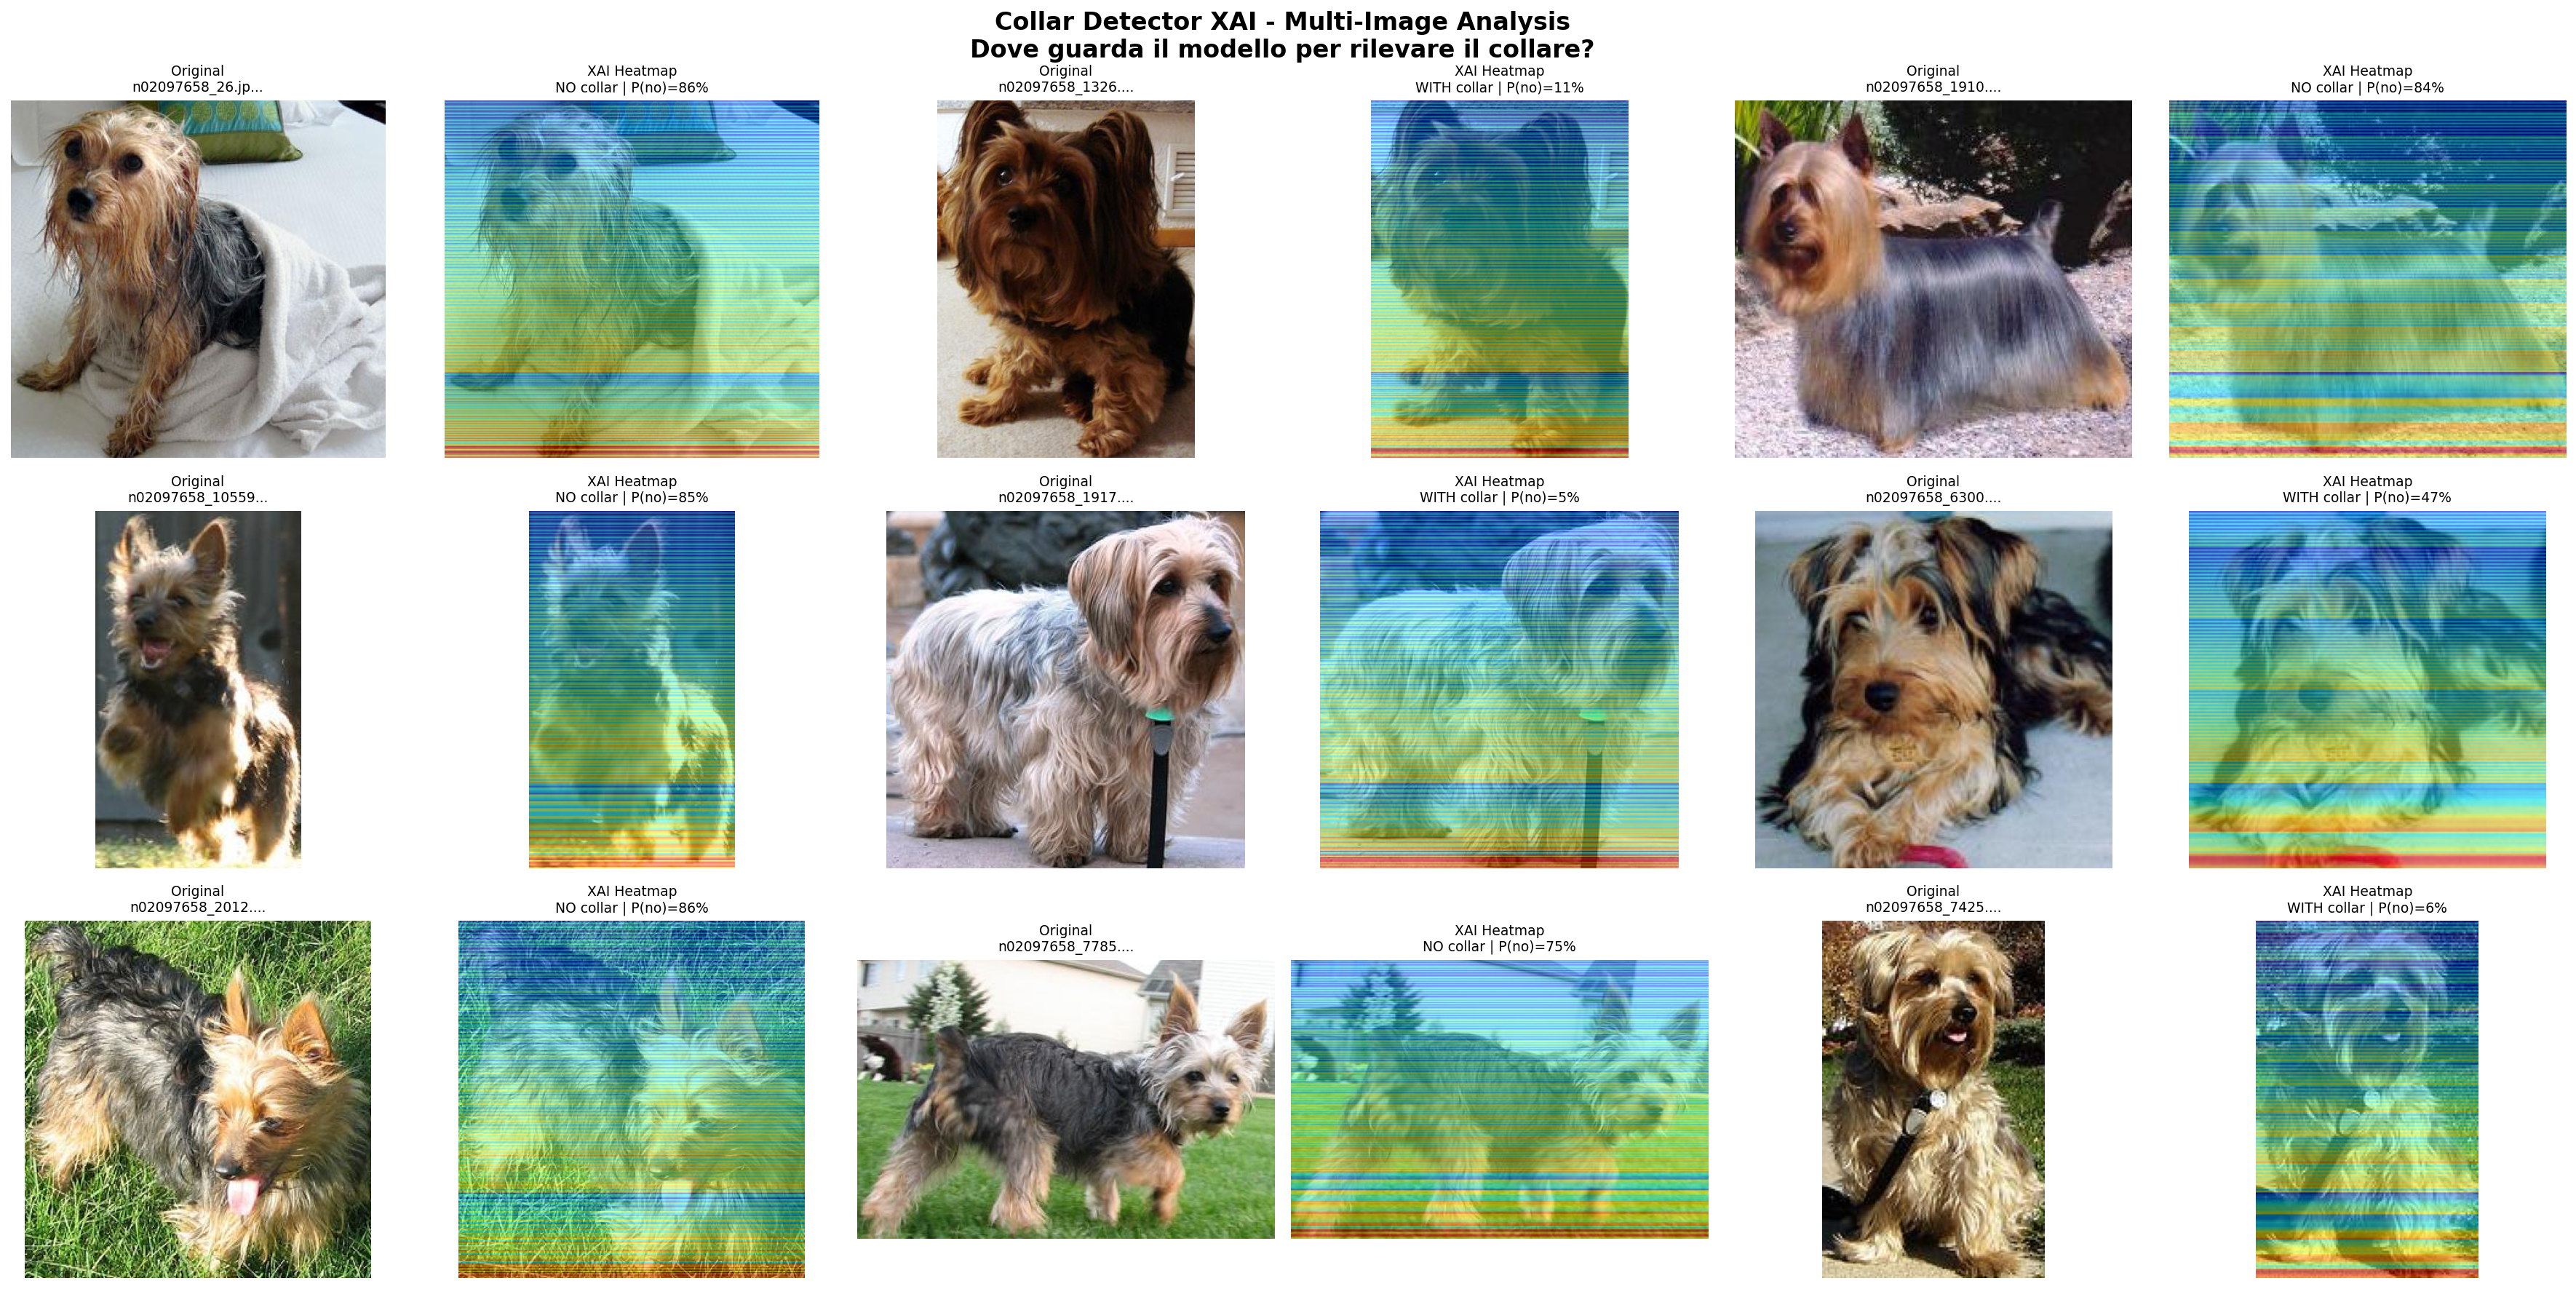
\includegraphics[width=\textwidth]{figures/collar_xai_multi_image.png}
    \caption{Analisi XAI del Collar Detector su diverse immagini. Per ogni coppia: immagine originale (sinistra) e heatmap di attenzione (destra). \textbf{Osservazione critica}: le zone calde sono spesso concentrate sulla parte inferiore dell'immagine (pavimento/erba) invece che sulla regione del collo.}
    \label{fig:collar_xai}
\end{figure}

\paragraph{Interpretazione:} Questo suggerisce che il modello potrebbe aver appreso \textbf{correlazioni spurie} dal dataset:
\begin{itemize}
    \item I cani \textbf{con collare} nel dataset potrebbero essere prevalentemente fotografati su superfici specifiche (es. pavimento domestico, marciapiede)
    \item I cani \textbf{senza collare} potrebbero essere prevalentemente in contesti diversi (es. erba, terra battuta)
    \item Il modello ha imparato a predire la presenza del collare basandosi sullo \textbf{sfondo} invece che sul collare stesso
\end{itemize}

\subsubsection{Analisi GradCAM Class-Specific}

Per confermare l'ipotesi del bias, \`e stata condotta un'analisi GradCAM separata per ciascuna classe di output, utilizzando la libreria \texttt{pytorch-grad-cam}.

\begin{figure}[H]
    \centering
    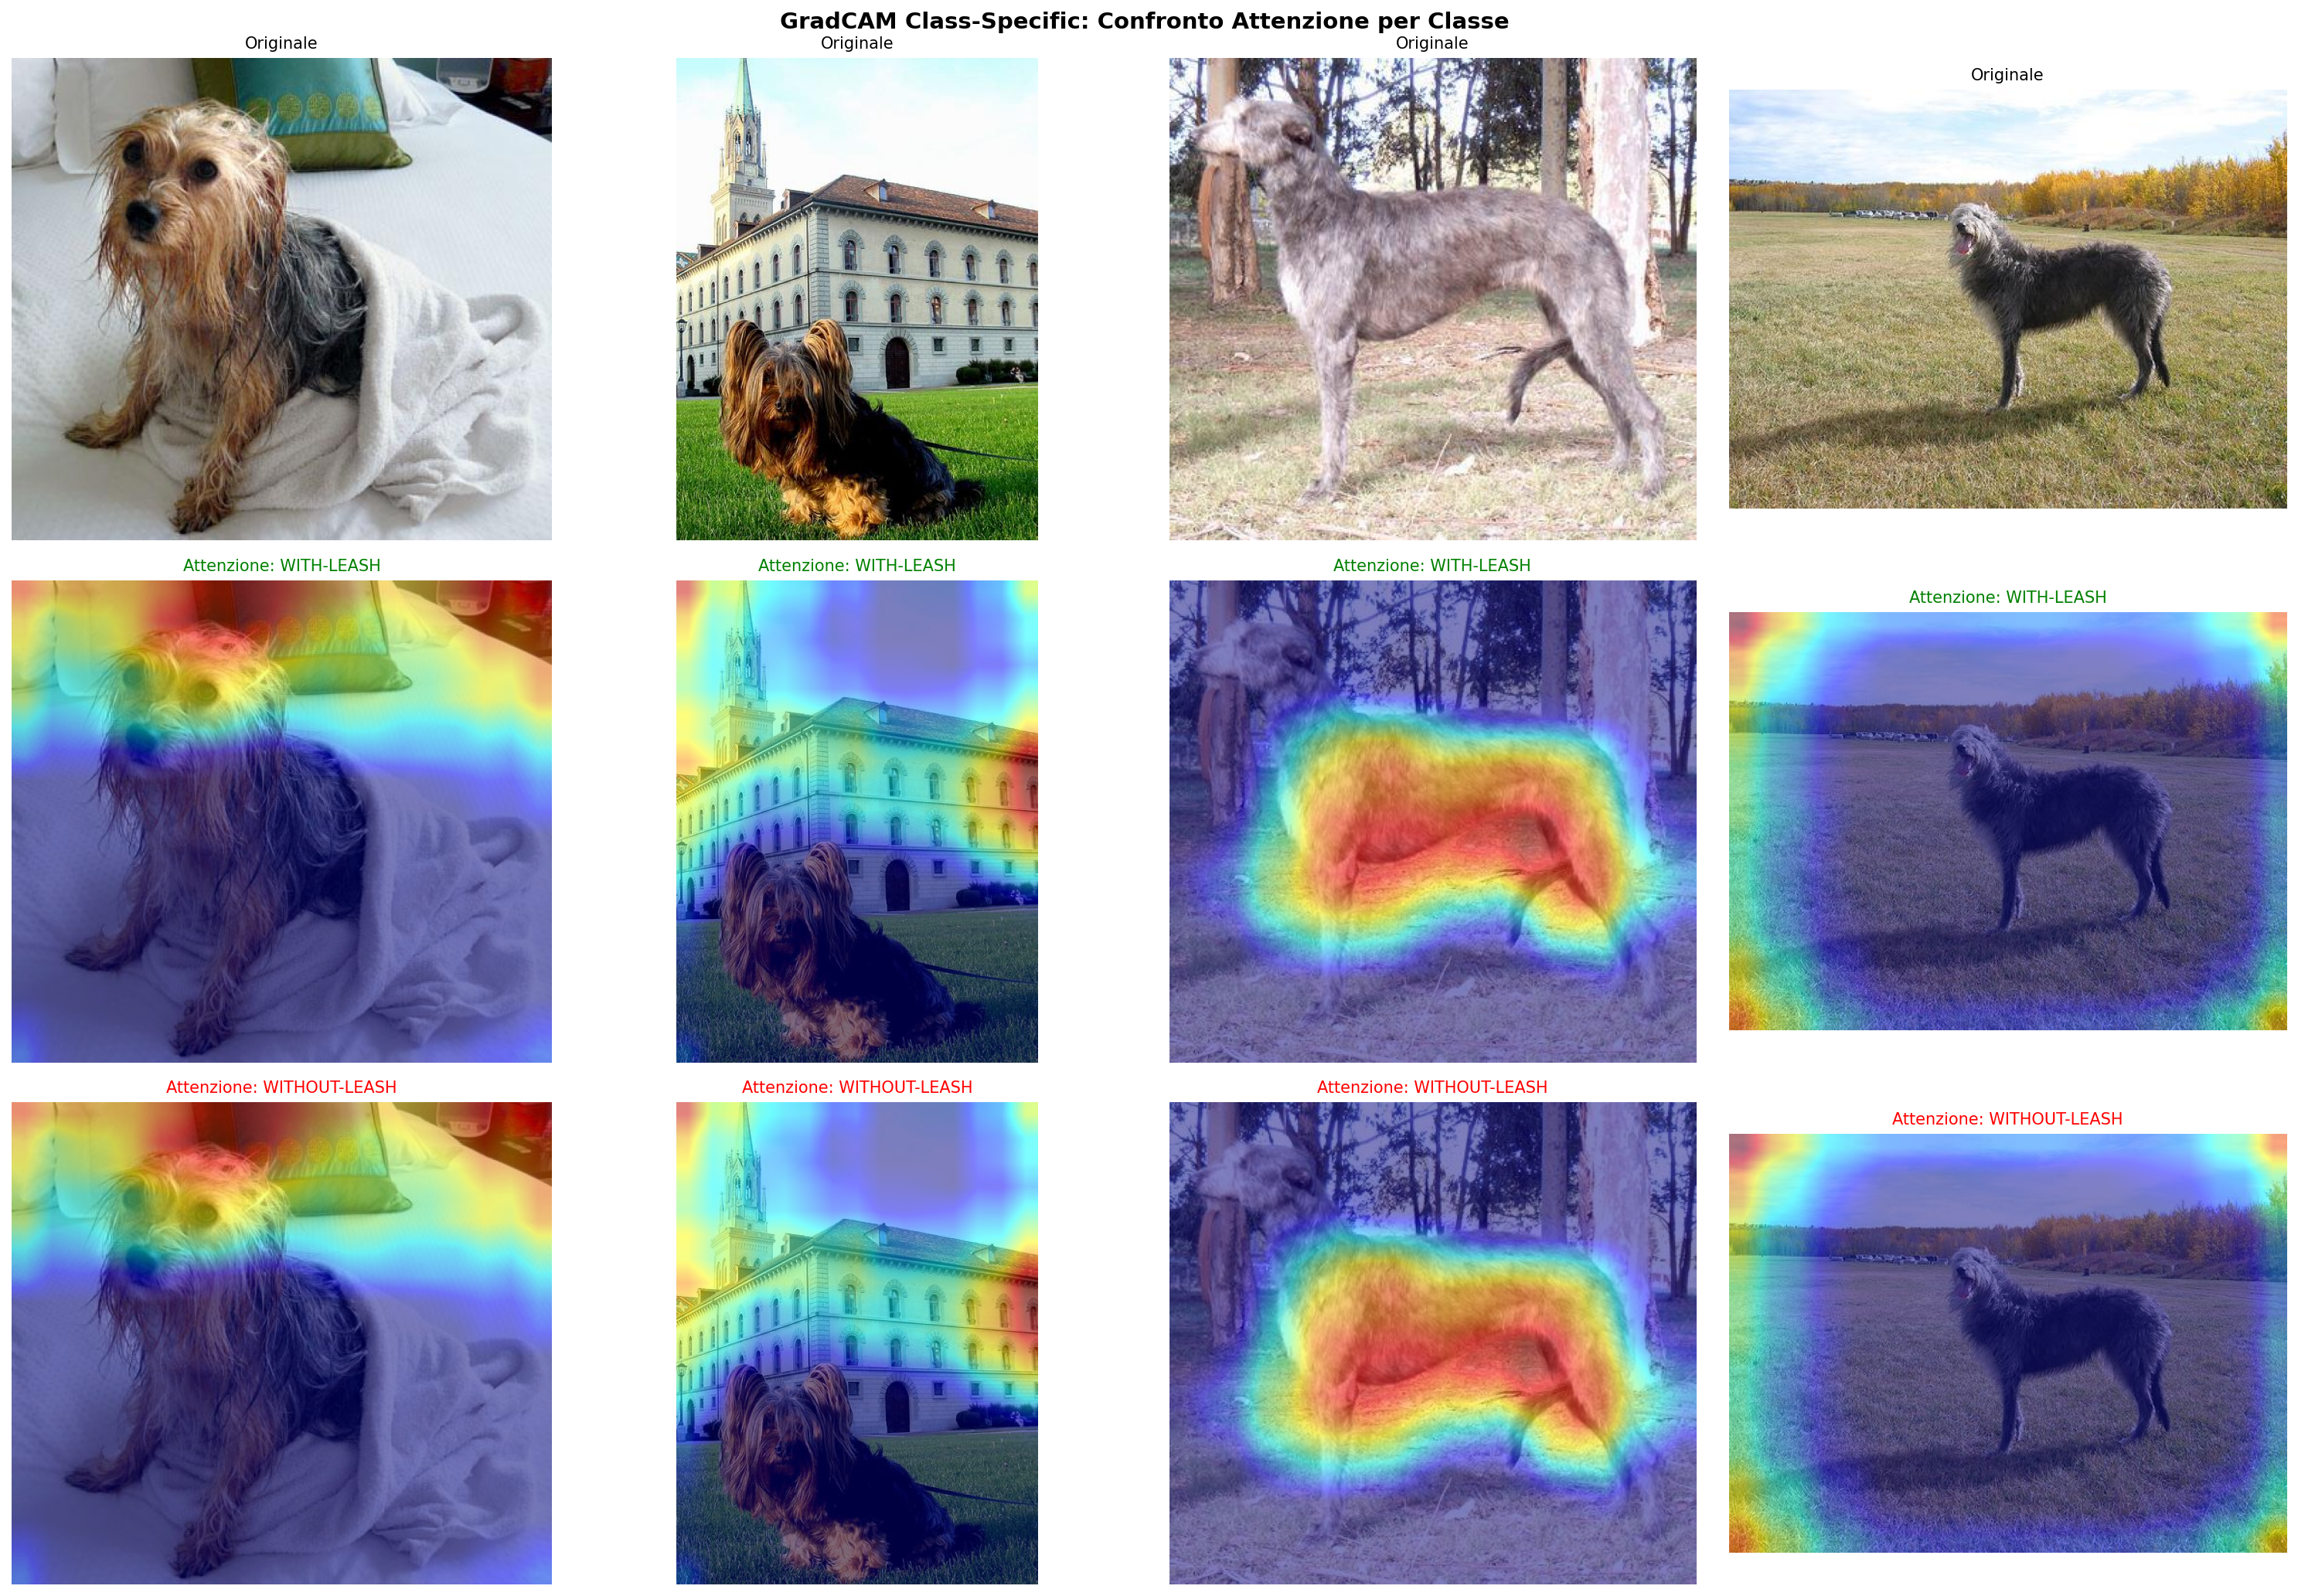
\includegraphics[width=\textwidth]{figures/collar_gradcam_class_comparison.png}
    \caption{Confronto GradCAM class-specific su immagini Stanford Dogs. Riga 1: immagini originali. Riga 2: mappa di attenzione per classe ``Dog-with-Leash''. Riga 3: mappa di attenzione per classe ``Dog-without-Leash''. Le heatmap sono \textbf{quasi identiche} tra le due classi.}
    \label{fig:collar_gradcam_comparison}
\end{figure}

\paragraph{Risultato Critico:} L'analisi class-specific rivela un problema fondamentale:

\begin{itemize}
    \item Le mappe di attenzione per \textbf{entrambe le classi sono identiche}
    \item L'attenzione \`e concentrata sul \textbf{corpo centrale} del cane, non sulla regione del collo
    \item Il modello non mostra \textbf{nessuna differenza} nel pattern di attenzione tra ``cercare il collare'' e ``verificare l'assenza del collare''
\end{itemize}

\paragraph{Interpretazione:} Un Collar Detector correttamente addestrato dovrebbe mostrare:
\begin{itemize}
    \item Per \textbf{Dog-with-Leash}: focus sulla zona \textbf{collo/collare}
    \item Per \textbf{Dog-without-Leash}: focus sulla zona \textbf{collo} per verificarne l'assenza
\end{itemize}

Il fatto che le heatmap siano identiche suggerisce che la decisione di classificazione avviene basandosi su \textbf{features non discriminative} (probabilmente correlazioni spurie con lo sfondo o il contesto), confermando il dataset bias ipotizzato.

\subsubsection{Implicazioni}

Nonostante il Collar Detector raggiunga un mAP@0.5 di 0.853 sul validation set, questo finding solleva dubbi sulla \textbf{generalizzazione} del modello:
\begin{itemize}
    \item Il modello potrebbe fallire su immagini dove lo sfondo non correla con la presenza del collare
    \item In deployment reale, le condizioni ambientali potrebbero differire significativamente dal training set
    \item \`E necessario un dataset pi\`u bilanciato in termini di contesti/sfondi
\end{itemize}

\paragraph{Azione Correttiva Proposta:} Per le versioni future, si propone di:
\begin{enumerate}
    \item Aumentare la variet\`a di sfondi nel dataset di training
    \item Applicare augmentation pi\`u aggressivo sullo sfondo (random background replacement)
    \item Utilizzare tecniche di object-centric learning per forzare l'attenzione sulla regione del collo
\end{enumerate}

\subsection{Backbone YOLO11: Keypoint Reliability}

Per il backbone di pose estimation, l'analisi si \`e concentrata sulla \textbf{affidabilit\`a dei keypoints} per gruppo anatomico.

\subsubsection{Analisi per Gruppo Anatomico}

I 24 keypoints sono stati raggruppati in categorie anatomiche:

\begin{figure}[H]
    \centering
    \includegraphics[width=\textwidth]{figures/backbone_keypoint_reliability.png}
    \caption{Analisi dell'affidabilit\`a dei keypoints. A sinistra: distribuzione della confidenza media per keypoint. A destra: matrice di correlazione tra gruppi anatomici.}
    \label{fig:backbone_reliability}
\end{figure}

\begin{table}[H]
\centering
\begin{tabular}{lcc}
\toprule
\textbf{Gruppo} & \textbf{Keypoints} & \textbf{Confidenza Media} \\
\midrule
Testa (nose, eyes, ears) & 5 & Alta ($> 0.8$) \\
Torso (withers, throat, tailbase) & 3 & Alta ($> 0.75$) \\
Zampe anteriori & 8 & Media ($\sim 0.6$) \\
Zampe posteriori & 8 & Media ($\sim 0.55$) \\
\bottomrule
\end{tabular}
\caption{Affidabilit\`a media dei keypoints per gruppo anatomico.}
\label{tab:keypoint_reliability}
\end{table}

\paragraph{Osservazioni:}
\begin{itemize}
    \item I keypoints della \textbf{testa} sono i pi\`u affidabili (sempre visibili)
    \item Le \textbf{zampe} hanno confidenza pi\`u variabile (occlusioni frequenti)
    \item Il Pose Classifier \`e robusto a queste variazioni grazie alla normalizzazione dei keypoints
\end{itemize}

\subsection{Pose Classifier: SHAP Analysis}

SHAP (SHapley Additive exPlanations) \cite{lundberg2017shap} fornisce spiegazioni a livello di feature per modelli tabellari come l'MLP del Pose Classifier.

\subsubsection{Features pi\`u Influenti}

L'analisi SHAP ha identificato le features pi\`u discriminanti per la classificazione stray/owned:

% Figura SHAP non disponibile - analisi testuale inclusa sotto
% \begin{figure}[H]
%     \centering
%     \includegraphics[width=\textwidth]{figures/pose_xai_multi_image.png}
%     \caption{Visualizzazione SHAP del Pose Classifier.}
%     \label{fig:pose_xai}
% \end{figure}

\begin{enumerate}
    \item \textbf{Posizione relativa della coda} (tailbase\_y normalizzato)
    \item \textbf{Apertura delle zampe posteriori} (distanza tra back\_left\_paw e back\_right\_paw)
    \item \textbf{Postura della testa} (nose\_y rispetto a withers\_y)
\end{enumerate}

\paragraph{Interpretazione:}
\begin{itemize}
    \item Coda bassa/tra le zampe $\rightarrow$ indica stress/paura (comune nei randagi)
    \item Zampe ravvicinate $\rightarrow$ postura difensiva
    \item Testa abbassata $\rightarrow$ sottomissione o ricerca di cibo
\end{itemize}

Questi pattern sono coerenti con la letteratura sul comportamento canino \cite{overall2013canine}, validando l'approccio weak supervision.

\subsection{Riepilogo e Raccomandazioni}

\begin{table}[H]
\centering
\begin{tabular}{lcp{5cm}}
\toprule
\textbf{Modello} & \textbf{XAI Status} & \textbf{Azione Raccomandata} \\
\midrule
Breed Classifier & \checkmark Corretto & Nessuna \\
Collar Detector & $\times$ \textbf{Bias grave} & Retraining con dataset bilanciato e ROI cropping su zona collo \\
Backbone YOLO11 & \checkmark Corretto & Nessuna \\
Pose Classifier & \checkmark Corretto & Nessuna \\
\bottomrule
\end{tabular}
\caption{Riepilogo analisi XAI e azioni raccomandate.}
\label{tab:xai_summary}
\end{table}

\paragraph{Conclusione:} L'analisi XAI ha rivelato che tre modelli su quattro utilizzano features semanticamente appropriate. Il \textbf{Collar Detector presenta un bias critico} confermato dall'analisi GradCAM class-specific: le mappe di attenzione identiche per entrambe le classi indicano che il modello non ha appreso a distinguere la presenza/assenza del collare guardando la regione anatomica corretta. Nonostante le buone metriche sul validation set (mAP 0.853), questo finding solleva seri dubbi sulla generalizzazione del modello in scenari reali. L'analisi XAI si \`e dimostrata fondamentale per identificare questo problema, che non sarebbe emerso dalle sole metriche quantitative.



% ============================================
% SEZIONE 11: IMPLEMENTAZIONE
% ============================================

\section{Implementazione}
\label{sec:implementazione}

\subsection{Stack Tecnologico}

\begin{table}[H]
\centering
\begin{tabular}{ll}
\toprule
\textbf{Componente} & \textbf{Tecnologia} \\
\midrule
Backend & Flask 3.0 + Flask-SocketIO \\
Frontend & React 18 + Vite + TailwindCSS \\
ML Framework & PyTorch + Ultralytics \\
Real-time & WebSocket (Socket.IO) \\
Database & SQLite (alert storage) \\
\bottomrule
\end{tabular}
\caption{Stack tecnologico del sistema}
\end{table}

\subsection{Backend Flask}

Il backend implementa:
\begin{itemize}
    \item REST API per upload e analisi immagini
    \item WebSocket per streaming real-time
    \item Sistema di alert con cooldown
    \item Persistenza degli alert su SQLite
\end{itemize}

\subsection{Frontend React}

L'interfaccia utente include:
\begin{itemize}
    \item Grid 2x2 di telecamere simulate
    \item Overlay con bounding box e Stray Index
    \item Pannello alert real-time
    \item Statistiche live (detections, avg SI, etc.)
\end{itemize}

% ============================================
% SEZIONE 12: PERCORSO DI SVILUPPO
% ============================================

\section{Il Percorso di Sviluppo}
\label{sec:percorso}

Questa sezione documenta il percorso iterativo seguito durante lo sviluppo di ResQPet, evidenziando le sfide affrontate, le soluzioni adottate e le lezioni apprese.

\subsection{Fase 1: La Sfida dei Dati}

Il primo ostacolo significativo \`e emerso con il Collar Detector. Il dataset iniziale (Roboflow ``Dog with Leash'') conteneva solo 152 immagini, producendo un modello con mAP del 51\% --- completamente inadeguato per un'applicazione reale.

\paragraph{Il problema:} I dataset pubblici per la detection di collari/guinzagli erano scarsi e di bassa qualit\`a. Le alternative erano:
\begin{enumerate}
    \item Cercare altri dataset pubblici (risultato: nessuno adeguato)
    \item Annotare manualmente migliaia di immagini (costo proibitivo)
    \item Costruire una soluzione custom
\end{enumerate}

\paragraph{La soluzione:} Abbiamo sviluppato una \textbf{piattaforma di labeling web} con approccio \textit{human-in-the-loop}:
\begin{itemize}
    \item Il modello v1 (seppur scadente) generava pre-annotazioni automatiche
    \item Gli annotatori umani dovevano solo \textit{verificare e correggere}, non annotare da zero
    \item Sistema multi-utente per parallelizzare il lavoro
\end{itemize}

\paragraph{Risultato:} Da 152 a 7,576 immagini annotate, con un miglioramento del \textbf{67\%} sul mAP (da 0.51 a 0.853). La lezione chiave: \textit{investire nei dati paga pi\`u che complicare il modello}.

\subsection{Fase 2: L'Intuizione della Weak Supervision}

La classificazione della postura presentava una sfida diversa: come definire oggettivamente una ``postura da randagio''?

\paragraph{Il problema:} L'annotazione manuale della postura \`e intrinsecamente soggettiva. Annotatori diversi avrebbero prodotto label inconsistenti, e il costo sarebbe stato elevato per migliaia di pose.

\paragraph{L'intuizione:} Invece di annotare \textit{come} appare una postura, sfruttiamo \textit{da dove} proviene l'immagine:
\begin{itemize}
    \item I cani nel FYP Dataset sono randagi \textit{per definizione}
    \item I cani in Stanford Dogs sono in contesti domestici/esposizioni
    \item L'origine del dataset diventa il label
\end{itemize}

\paragraph{Validazione:} L'approccio ha prodotto un AUC-ROC di 0.78, dimostrando che il segnale \`e informativo nonostante il label noise intrinseco. La weak supervision ha permesso di creare un dataset di oltre 30,000 keypoints senza alcuna annotazione manuale.

\subsection{Fase 3: Integrazione e Bilanciamento}

L'ultima sfida \`e stata combinare i quattro classificatori in modo bilanciato.

\paragraph{Il problema:} Come pesare indicatori con affidabilit\`a diverse? Il collar detector (mAP 85\%) \`e pi\`u affidabile del pose classifier (AUC 78\%), ma entrambi forniscono informazioni utili.

\paragraph{La soluzione:} Pesi empirici basati su:
\begin{itemize}
    \item \textbf{Collar (35\%)}: Indicatore pi\`u diretto e affidabile
    \item \textbf{Pose (25\%)}: Informativo ma rumoroso (weak supervision)
    \item \textbf{Skin (20\%)}: Indicatore di trascuratezza
    \item \textbf{Breed (20\%)}: Prior statistici di supporto
\end{itemize}

La somma pesata produce uno Stray Index continuo che permette di gestire l'incertezza attraverso soglie configurabili.

\subsection{Lezioni Apprese}

\begin{enumerate}
    \item \textbf{Dati $>$ Modello}: Lo stesso YOLOv8n con 50$\times$ pi\`u dati ha migliorato del 67\%. La qualit\`a dei dati \`e pi\`u importante della complessit\`a del modello.

    \item \textbf{Human-in-the-loop}: Combinare automazione (pre-labeling) e supervisione umana (verifica) \`e pi\`u efficiente dell'annotazione manuale pura.

    \item \textbf{Weak supervision funziona}: Con assunzioni ragionevoli sulla provenienza dei dati, si possono ottenere risultati utili senza annotazione manuale.

    \item \textbf{Iterazione}: Il ``fallimento'' del collar v1 ha accelerato la creazione del dataset v2 attraverso il pre-labeling. I fallimenti sono parte del processo.

    \item \textbf{Trasparenza}: Uno Stray Index continuo \`e pi\`u utile di una classificazione binaria, perch\'e permette di calibrare il trade-off tra falsi positivi e negativi.
\end{enumerate}

% ============================================
% SEZIONE 13: DISCUSSIONE
% ============================================

\section{Discussione}
\label{sec:discussione}

\subsection{Punti di Forza}
\begin{itemize}
    \item Architettura modulare e estendibile
    \item Approccio weak supervision innovativo per pose classification
    \item \textbf{Piattaforma di labeling custom}: Sviluppata per creare il dataset collar v2 (50$\times$ pi\`u dati)
    \item \textbf{Human-in-the-loop}: Pre-labeling automatico + revisione umana per dataset di qualit\`a
    \item Interfaccia utente intuitiva
    \item Pipeline end-to-end funzionante con 28 FPS su GPU
\end{itemize}

\subsection{Limitazioni}
\begin{itemize}
    \item Breed priors basati su stime, non su dati reali italiani
    \item Performance dipendente dalla qualit\`a delle immagini
    \item Assumption che la postura sia correlata allo stato di abbandono
    \item Validazione umana limitata a 133 immagini (da estendere)
    \item \textbf{Dataset bias nel Collar Detector}: L'analisi XAI (Sezione~\ref{sec:collar_bias}) ha rivelato che il modello presta attenzione allo sfondo invece che alla regione del collare, suggerendo correlazioni spurie nel dataset di training
\end{itemize}

\subsection{Sviluppi Futuri}
\begin{itemize}
    \item Integrazione con database nazionali di cani smarriti
    \item Supporto per stream video reali
    \item Aggiunta di facial recognition per re-identificazione
    \item Validazione su dati reali da canili
    \item \textbf{Mitigazione dataset bias}: Ribilanciamento del dataset Collar con maggiore variet\`a di sfondi e tecniche di augmentation mirate
\end{itemize}

% ============================================
\section{Conclusioni}
% ============================================

Questo lavoro ha presentato ResQPet, un sistema di identificazione automatizzata dello stato di abbandono nei cani. Il contributo principale è l'introduzione di un approccio di weak supervision per la classificazione della postura, che elimina la necessità di annotazione manuale sfruttando l'origine dei dataset.

Il sistema combina quattro classificatori specializzati attraverso una fusione pesata, producendo uno Stray Index che quantifica la probabilità di abbandono. L'implementazione include un'interfaccia web che simula un sistema CCTV per il monitoraggio real-time.

I risultati preliminari mostrano la fattibilità dell'approccio, sebbene siano necessarie ulteriori validazioni su dati reali per confermare l'efficacia del sistema in scenari operativi.

% ============================================
% Bibliography
% ============================================

\bibliographystyle{plain}
\bibliography{bibliography}

% ============================================
\appendix
\section{Appendice A: Dettagli Dataset}
% ============================================

\begin{table}[H]
\centering
\begin{tabular}{lllll}
\toprule
\textbf{Dataset} & \textbf{Immagini} & \textbf{Classi} & \textbf{Fonte} & \textbf{Uso} \\
\midrule
Dog-Pose & 8,476 & 1 + 24kpt & Ultralytics & Backbone \\
Collar (v2) & 7,576 & 2 & Labeling Platform & Collar Detector \\
Dog's Skin Diseases & 4,315 & 6 & Kaggle & Skin Classifier \\
Stanford Dogs & $\sim$20,000 & 120 & Stanford & Breed + Labeling \\
FYP Stray Dogs & $\sim$20,000 & 4 & Custom & Pose Classifier \\
\bottomrule
\end{tabular}
\caption{Riepilogo dataset utilizzati. Il dataset Collar v2 \`e stato creato attraverso la piattaforma di labeling custom.}
\end{table}

% ============================================
\section{Appendice B: Hyperparameters}
% ============================================

\subsection{Backbone YOLO11 Dog-Pose v2}
\begin{table}[H]
\centering
\begin{tabular}{ll}
\toprule
\textbf{Parametro} & \textbf{Valore} \\
\midrule
Epochs & 150 \\
Batch size & 16 \\
Image size & 640$\times$640 \\
Optimizer & AdamW \\
LR iniziale & 0.001 \\
LR finale & 0.01 \\
Weight decay & 0.0005 \\
Early stopping & 20 epochs \\
\bottomrule
\end{tabular}
\end{table}

\subsection{Collar Detector v2}
\begin{table}[H]
\centering
\begin{tabular}{ll}
\toprule
\textbf{Parametro} & \textbf{Valore} \\
\midrule
Epochs & 100 \\
Batch size & 128 (64/GPU) \\
Image size & 640$\times$640 \\
Optimizer & AdamW \\
LR iniziale & 0.001 \\
Device & 2$\times$ RTX 5090 \\
Mixed Precision & FP16 \\
Augmentation & Mosaic, MixUp, HSV, Flip \\
\bottomrule
\end{tabular}
\end{table}

% ============================================
\section{Appendice C: Guida Installazione}
% ============================================

Per le istruzioni di installazione aggiornate, consultare il file \texttt{README.md} e \texttt{TRAINING\_SETUP.md} nel repository ufficiale:

\begin{center}
\url{https://github.com/GrandeVx/ResQPet}
\end{center}

Il repository include:
\begin{itemize}
    \item Istruzioni di setup backend e frontend
    \item Link per download dei weights pre-trainati (Google Drive)
    \item Requisiti hardware e software
    \item Guida per ri-training dei modelli da zero
\end{itemize}

\end{document}
